\documentclass[12pt, twoside]{article}
\usepackage[utf8]{inputenc}
\usepackage[english]{babel}

\usepackage{amsthm}
\usepackage{a4wide}
\usepackage{graphicx}
\usepackage{caption}
\usepackage{amssymb}
\usepackage{amsmath}
\usepackage{mathrsfs}
\usepackage{euscript}
\usepackage{graphicx}
\usepackage{subfig}
\usepackage{caption}
\usepackage{color}
\usepackage{bm}
\usepackage{tabularx}
\usepackage{adjustbox}


\usepackage[toc,page]{appendix}

\usepackage{comment}
\usepackage{rotating}

\DeclareMathOperator*{\argmax}{arg\,max}
\DeclareMathOperator*{\argmin}{arg\,min}

\newtheorem{theorem}{Theorem}
\newtheorem{lemma}[theorem]{Lemma}
\newtheorem{definition}{Definition}[section]

%\numberwithin{equation}{section}

\newcommand*{\No}{No.}

\usepackage{autonum}

\begin{document}

\title{\bf Prior distribution choices for a mixture of experts \thanks{This research was supported by RFBR (project ???) and NTI (project ???).}}
\date{}
\author{}
\maketitle

\begin{center}
\bf
A. V. Grabovoy\footnote{Moscow Institute of Physics and Technology, grabovoy.av@phystech.edu},
V. V. Strijov\footnote{Moscow Institute of Physics and Technology, Dorodnicyn Computing Centre, Federal Research Center “Computer Science and Control” of the Russian Academy of Sciences, strijov@phystech.edu}
\end{center}
{\centering\begin{quote}
\textbf{Abstract:} 
The paper investigates a mixture of expert models. 
The mixture of experts is a set of experts and the gate function which weighs these experts. Each expert is a linear model.
The gate function is a neural network with softmax on the last layer. 
The paper analyzes different prior distributions for each expert.
The authors propose a method that takes into account the relationship between the prior distributions of different experts.
The paper uses the EM algorithm for solving the optimization problem.
This paper proposes to use the mixture of experts for the problem of circles parameters estimation.
Each expert fits one circle in the image.
The experiment uses synthetic and real data to test the proposed method.
The real data is a human eye image from the iris detection problem.


\smallskip
\textbf{Keywords}: mixture of Experts; bayesian model selection; prior distribution.

\smallskip
\end{quote}
}

\section{Introduction}
The paper studies the problem of a mixture of experts constructing. A mixture of experts is multimodel, which are weighed local models that approximate the dataset. The weighting coefficients depend on datum from the dataset.

Examples of multimodel are bagging, gradient boosting~\cite{Tianqi2016} and random forest~\cite{Ishwaran2012}. There are approaches to multimodeling~\cite{Yuksel2012} suggests that the contribution of each expert to the answer depends on the object from the dataset. A mixture of experts uses a gate function that weights the prediction of each expert.

The main problem of multimodal is a convergence dependence on the initial point.
We are using the probability approach for finding optimal mixture parameters and local expert parameters.
The paper proposes to use different prior distribution for the parameters to improve convergence.
The paper introduces the method which is using a dependence between prior distribution to improve multimodel quality.

\begin{figure}[h!t]\center
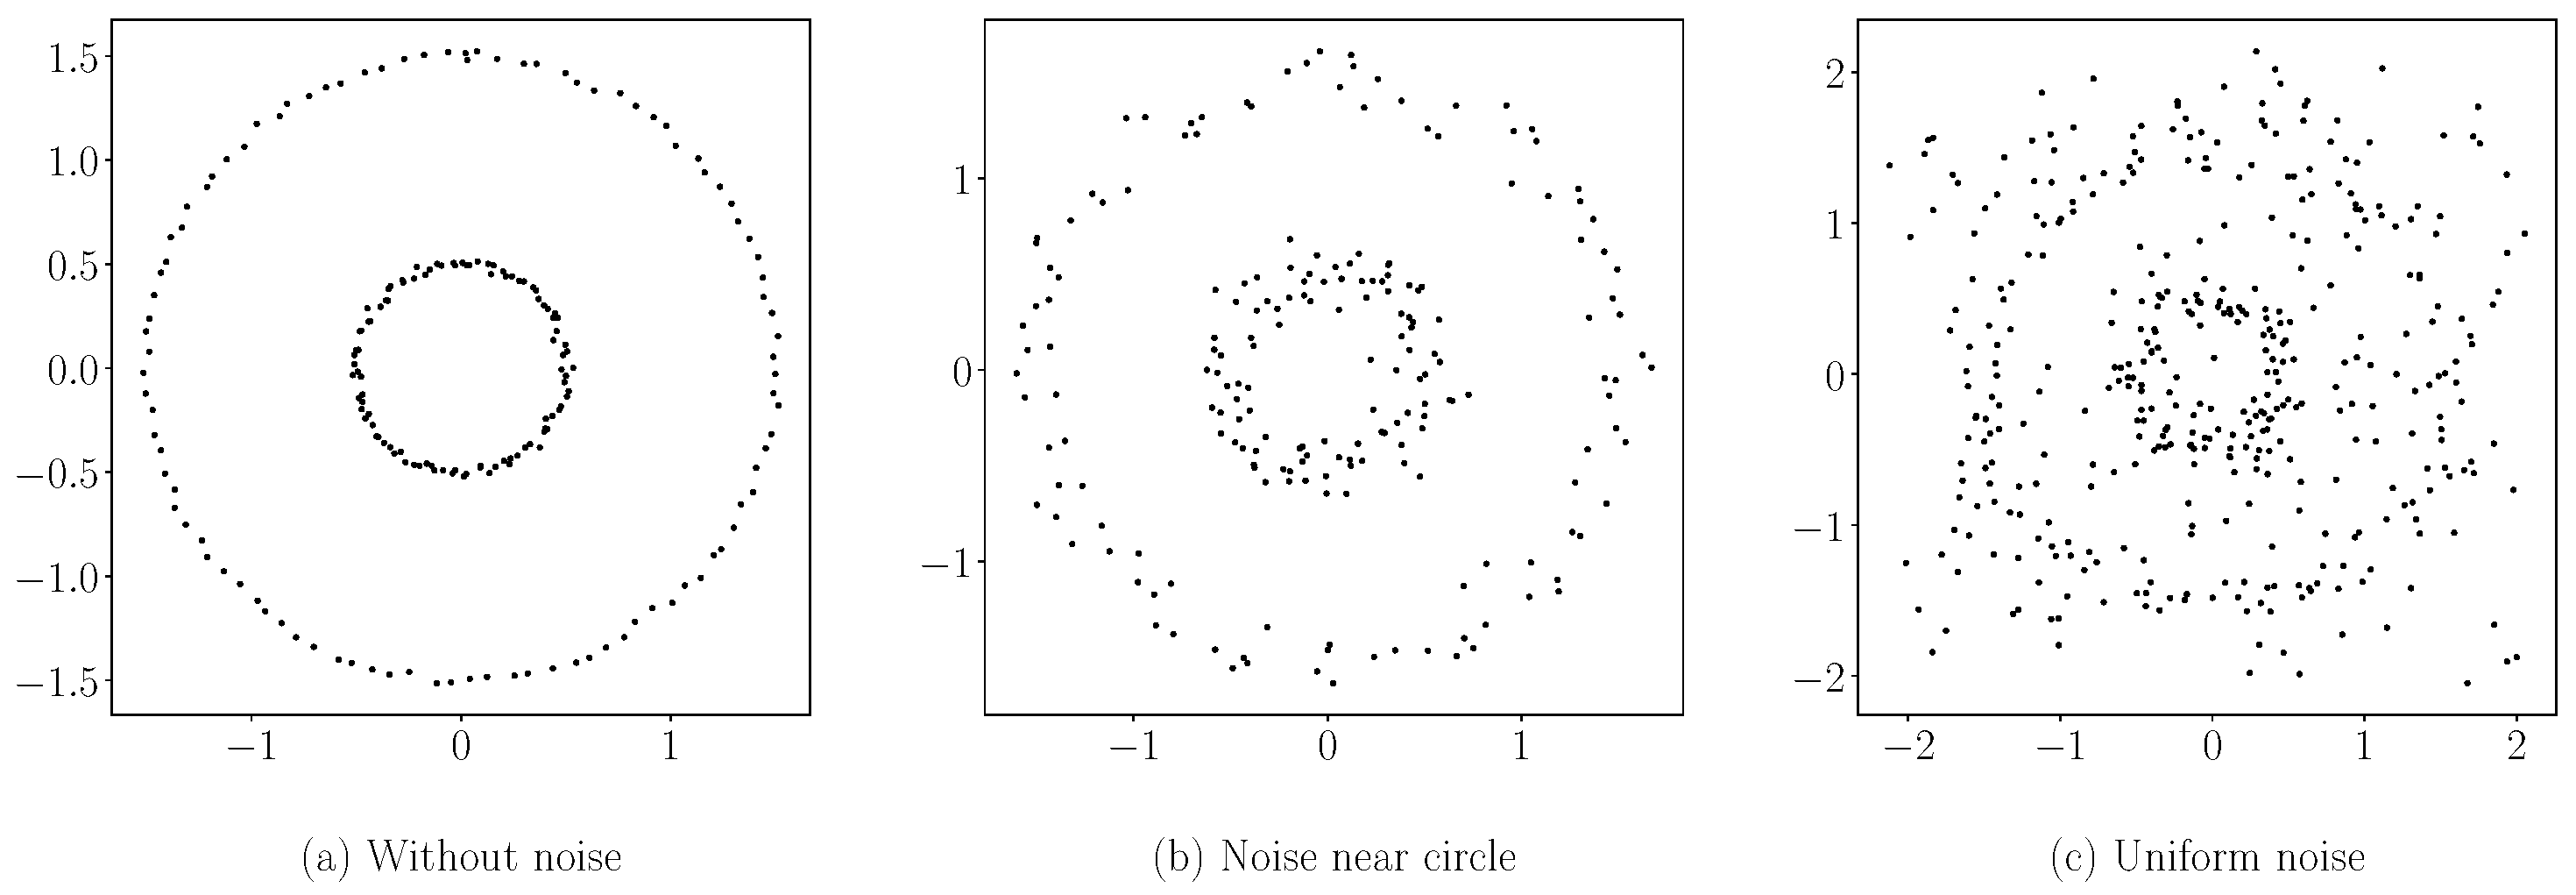
\includegraphics[width=1\textwidth]{result_eng/statment}
\caption{An example of circles with different noise levels: (a) circle without noise; (b) noisy radius circle; (c) noisy radius circle, and uniform noisy on image}
\label{example:1}
\end{figure}

The paper analysis multimodel quality depending on the prior distribution for the expert's parameters.
There solves a problem of finding circles on a binarized image.
Examples of images are shown in fig.~\ref{example:1}.
In this paper, each expert is a linear model.
A gate function is a two-layer fully connected neural network.

\section{Related work}
Many papers on a mixture of experts are devoted to the choice of a gateway function: softmax, the Dirichlet process~\cite{Edward2002}, a neural network~\cite{Shazeer2017} with softmax function on the last layer.
Some papers are devoted to the choice of expert type. 
Papers~\cite{Jordan1994, Jordan1991} analyze linear models as experts.
Papers~\cite{Lima2007, Cao2003} analyze SVMs as experts.
The paper~\cite{Yuksel2012} contains an overview of different methods for choosing a gate function and expert type.

A mixture of experts has many applications.
Papers~\cite{Yumlu2003, Cheung1995, Weigend2000} use a mixture of experts in the task of forecasting time series.
The paper~\cite{Ebrahimpour2009} uses a mixture of experts in the task of recognizing handwritten numbers.
Papers~\cite{Estabrooks2001, Mossavat2010, Peng1996, Tuerk2001}  are devoted to methods of text and speech recognition by using a mixture of experts.
The paper~\cite{Sminchisescu2007} analyzes a mixture of experts in the task of recognizing three-dimensional human movements.

The paper~\cite{Bowyer2010} is devoted to a review of the study results on the iris detection in the image.
The methods of highlighting the borders of the iris and pupil are described in papers~\cite{Matveev2010, Matveev2014}.

\section{Problem statement of circle parameters estimation}
This data are binary image
\[
\label{eq:st:cr:1}
\begin{aligned}
\textbf{M} \in \{0,1\}^{m_1 \times m_2},
\end{aligned}
\]
where~$1$ is a black pixel, an image, and $0$ is a white pixel, the image background.
The image~$\textbf{M}$ is mapped to a set of coordinates~$\textbf{C}=\left\{x_i, y_i\right\}_{i=1}^{N}$. The pair of coordinates~$(x_i, y_i)$ is a black pixel in~$\textbf{M}$:
\[
\label{eq:st:cr:2}
\begin{aligned}
\textbf{C} \in  \mathbb{R}^{N \times 2},
\end{aligned}
\]
where~$N$ is the number of black pixels.

Let~$(x_0, y_0)$ be the center of the circle, and $r$ is radius of the circle.
 The coordinates $\left(x_i, y_i\right)\in\textbf{C}$ is a circle locus of points defined by
\[
\label{eq:st:cr:3}
\begin{aligned}
\left(x_i - x_0\right)^{2}+\left(y_i-y_0\right)^2 = r^2.
\end{aligned}
\]
Expand brackets:
\[
\label{eq:st:cr:4}
\begin{aligned}
(2x_0)\cdot x_i + (2y_0)\cdot y_i+(r^2-x_0^2-y_0^2)\cdot1 = x_{i}^2 + y_{i}^2.
\end{aligned}
\]
Rewrite equation~\eqref{eq:st:cr:4} to set the linear regressions problem for all points in the dataset:
\[
\label{eq:st:cr:5}
\begin{aligned}
\textbf{X}\textbf{w} \approx \textbf{y},  \quad \textbf{X} = \left[\textbf{C}, \textbf{1}\right], \quad \textbf{y} = [x_1^2+y_1^2, x_2^2+y_2^2, \cdots, x_N^2+y_N^2]^{\mathsf{T}}.
\end{aligned}
\]
The parameters~$\textbf{w} = \bigr[w_1, w_2, w_3\bigr]^{\mathsf{T}}$ reconstruct the circle parameters~$x_0, y_0, r$:
\[
\label{eq:st:cr:6}
\begin{aligned}
x_0 = \frac{w_1}{2}, \quad y_0 = \frac{w_2}{2}, \quad r = \sqrt[]{w_3+x_{0}^{2}+y_{0}^{2}}.
\end{aligned}
\]
The solution of problem~\eqref{eq:st:cr:5} reconstructs the circle parameters only if the number of circles in an image is equal to one.
The authors propose to use the multimodel for the image, which consists of several circles.
The multimodel is an ensemble of the linear models.
Each linear model approximates only one circle in the image.
In this paper, multimodel is a mixture of experts.

\section{Problem statement of building a mixture of experts}
\begin{definition}
\label{def:1}
A model~$\mathbf{f}$ is a local model on dataset~$\textbf{X}$ if~model $\mathbf{f}$ approximate some not empty subset~$\textbf{X}'\subset\textbf{X}$.
\end{definition}
Generalize one-circle approximation problem to the case of several circles.
Each circle is a local model.
The data for this case is
\[
\label{eq:st:1}
\begin{aligned}
\textbf{X} \in \mathbb{R}^{N \times n},
\end{aligned}
\]
where~$N$ is a number of datum and~$n$ is a number of features. In this paper,~$n$ is equal to 3.

\begin{definition}
\label{def:2}
Call the multimodel~$\hat{\mathbf{f}}$ a mixture of experts if
\[
\label{eq:st:2}
\begin{aligned}
\hat{\mathbf{f}} = \sum_{k=1}^{K}\pi_{k}\mathbf{f}_k, \qquad \pi_{k}\left(\mathbf{x}, \mathbf{V}\right):\mathbb{R}^{n\times \left|\mathbf{V}\right|} \to [0, 1], \qquad \sum_{k=1}^{K}\pi_{k}\left(\mathbf{x}, \mathbf{V}\right) = 1,
\end{aligned}
\]
where~$\mathbf{f}_k$ is a local model, $\pi_k$ is a gate function, vector~$\mathbf{w}_k$ is some parameters of the local model and~$\mathbf{V}$ is some parameters of the gate function.
\end{definition}

This paper asserts the local model a linear model. The gate function is the two--layer fully connected neural network
\[
\label{eq:st:3}
\begin{aligned}
\mathbf{f}_k\left(\textbf{x}\right) = \textbf{w}_k^{\mathsf{T}}\textbf{x}, \quad
\bm{\pi}\left(\mathbf{x}, \mathbf{V}\right) = \text{softmax}\bigr(\mathbf{V}_{1}^{\mathsf{T}}\bm{\sigma}\left(\mathbf{V}_2^{\mathsf{T}}\mathbf{x}\right)\bigr),
\end{aligned}
\]
where $\mathbf{V} = \bigr\{\mathbf{V}_1, \mathbf{V}_2\bigr\}$ is a set of the gate function parameters.

Combining~\eqref{eq:st:2} and~\eqref{eq:st:3}, obtain the likelihood solution:
\[
\label{eq:st:4}
\begin{aligned}
p\bigr(\mathbf{y}, \mathbf{W}|\mathbf{X}, \mathbf{V}\bigr) = \prod_{k=1}^{K}p^{k}\bigr(\mathbf{w}_k\bigr)\prod_{i=1}^{N}\left(\sum_{k=1}^{K}\pi_{k}p_{k}\bigr(y_i|\mathbf{w}_k, \mathbf{x}_i\bigr)\right),
\end{aligned}
\]
where~$\mathbf{W} = \bigr[\mathbf{w}_1, \mathbf{w}_2, \cdots, \mathbf{w}_K\bigr]^{\mathsf{T}}.$

The optimal parameters is delivered by the maximum likelihood solution:
\[
\label{eq:st:5}
\begin{aligned}
\hat{\mathbf{W}}, \hat{\mathbf{V}} = \arg\max_{\mathbf{W}, \mathbf{V}} p\bigr(\mathbf{y}, \mathbf{W}|\mathbf{X}, \mathbf{V}\bigr).
\end{aligned}
\]

\section{EM--algorithm as a solver of optimisation problem }
To build a mixture of experts, set the following probabilistic statement for the problem~\eqref{eq:st:1}:

\begin{enumerate}
	\item[1)] a likelihood $p_{k}\left(y_{i}|\mathbf{w}_{k}, \mathbf{x}_{i}\right) = \mathcal{N}\left(y_{i}|\mathbf{w}_{k}^{\mathsf{T}}\mathbf{x}_{i}, \beta^{-1}\right).$ Parameter~$\beta$ is a level of noise,
	\item[2)] a prior distribution for the parameters $p^{k}\left(\mathbf{w}_{k}\right) = \mathcal{N}\left(\mathbf{w}_{k}|\mathbf{w}^{0}_{k}, \mathbf{A}_{k}\right),$ where $\mathbf{w}^{0}_{k}$ is a vector of size $n\times1$ and~$\mathbf{A}_{k}$ is a covariance matrix,
	\item[3)] prior regularisation $p\left(\bm{\varepsilon}_{k,k'}|\bm{\Xi}\right) = \mathcal{N}\left(\bm{\varepsilon}_{k,k'}|\mathbf{0},  \bm{\Xi}\right),$ where~$\bm{\Xi}$ is a covariance matrix and $\bm{\varepsilon}_{k,k'} = \mathbf{w}_{k}^{0}-\mathbf{w}_{k'}^{0}.$
\end{enumerate}
Combining assumptions~$1), 2), 3)$ and equation~\eqref{eq:st:4}, obtain
\[
\label{eq:em:1}
\begin{aligned}
p\bigr(\mathbf{y}, \mathbf{W}|\mathbf{X}, \mathbf{V}, \textbf{A}, \textbf{W}^{0}, \bm{\Xi}, \beta\bigr) = &\prod_{k,k'=1}^{K}\mathcal{N}\left(\bm{\varepsilon}_{k,k'}|\mathbf{0},  \bm{\Xi}\right)\cdot\\
&\cdot\prod_{k=1}^{K}\mathcal{N}\left(\mathbf{w}_{k}|\mathbf{w}^{0}_{k}, \mathbf{A}_{k}\right)\prod_{i=1}^{N}\left(\sum_{k=1}^{K}\pi_{k}\mathcal{N}\left(y_{i}|\mathbf{w}_{k}^{\mathsf{T}}\mathbf{x}_{i}, \beta^{-1}\right)\right),
\end{aligned}
\]
 where~$\mathbf{A} = \bigr\{\mathbf{A}_1, \cdots, \mathbf{A}_K\bigr\}.$
 
Introduce a binary matrix~$\mathbf{Z}$. Its element~$z_{ik}$ is equal to $1$ if and only if the object $i$ is related to the local model $k$.
Integrating the binary matrix~$\mathbf{Z}$ in~\eqref{eq:em:1}, obtain:
\[
\label{eq:em:2}
\begin{aligned}
\log p\bigr(\mathbf{y}, \mathbf{Z}, \mathbf{W}&|\mathbf{X}, \mathbf{V}, \textbf{A}, \textbf{W}^{0},  \bm{\Xi}, \beta\bigr) =\\
&= \sum_{i=1}^{N}\sum_{k=1}^{K}z_{ik}\left[\log\pi_k\left(\textbf{x}_i, \textbf{V}\right) - \frac{\beta}{2}\left(y_{i} - \textbf{w}_{k}^{\mathsf{T}}\textbf{x}_{i}\right)^{2} + \frac{1}{2}\log\frac{\beta}{2\pi}\right] +\\
&+ \sum_{k=1}^{K}\left[-\frac{1}{2}\left(\textbf{w}_{k} - \textbf{w}_{k}^{0}\right)^{\mathsf{T}}\textbf{A}_{k}^{-1}\left(\textbf{w}_{k} - \textbf{w}_{k}^{0}\right) + \frac{1}{2}\log\det\textbf{A}^{-1}_{k} - \frac{n}{2}\log2\pi\right]+\\
&+ \sum_{k=1}^{K}\sum_{k'=1}^{K}\left[-\frac{1}{2}\left(\textbf{w}_{k}^{0}-\textbf{w}_{k'}^{0}\right)^{\mathsf{T}}\bm{\Xi}^{-1}\left(\textbf{w}_{k}^{0}-\textbf{w}_{k'}^{0}\right) +\frac{1}{2}\log\det \bm{\Xi} -\frac{n}{2}\log{2\pi}\right].
\end{aligned}
\]
Obtain a new optimisation problem combining~\eqref{eq:st:5} and~\eqref{eq:em:2}:
\[
\label{eq:em:3}
\begin{aligned}
\mathbf{W}, \mathbf{Z}, \mathbf{V}, \mathbf{W}^0, \textbf{A},  \beta = \arg\max_{\mathbf{W}, \mathbf{Z}, \mathbf{V}, \mathbf{W}^0, \textbf{A}, \beta} \log p\bigr(\mathbf{y}, \mathbf{Z}, \mathbf{W}&|\mathbf{X}, \mathbf{V}, \textbf{A}, \textbf{W}^{0}, \bm{\Xi}, \beta\bigr).
\end{aligned}
\]
Use the expectation-maximization~\cite{bishop2006} algorithm to find the maximum likelihood solution~\eqref{eq:em:3} for the multimodel~\eqref{eq:em:1} with latent variable~$\mathbf{Z}$.

\paragraph{E--step.} 
Let a join distribution~$q\left(\mathbf{Z}, \mathbf{W}\right)$ satisfies  the following assumption~$q\left(\mathbf{Z}, \mathbf{W}\right) = q\left(\mathbf{Z}\right)q\left(\mathbf{W}\right)$~\cite{bishop2006}. 
The symbol~$\propto$ means that both sides are equal to up to an additive constant.
First, find the distribution~$q\left(\textbf{Z}\right)$:
\[
\label{eq:em:4}
\begin{aligned}
\log q\left(\textbf{Z}\right) &= \mathsf{E}_{q/\textbf{Z}} \log p\bigr(\mathbf{y}, \mathbf{Z}, \mathbf{W}|\mathbf{X}, \mathbf{V}, \textbf{A}, \textbf{W}^{0}, \bm{\Xi}, \beta\bigr)  \propto\\
&\propto \sum_{i+1}^{N}\sum_{k=1}^{K}z_{ik}\left[\log\pi_{k}\left(\textbf{x}_{i}, \textbf{V}\right) - \frac{\beta}{2}\left(y_{i}^{2} -\textbf{x}_{i}^{\mathsf{T}}\mathsf{E}\textbf{w}_{k} + \textbf{x}_{i}^{\mathsf{T}}\mathsf{E}\textbf{w}_{k}\textbf{w}_{k}^{\mathsf{T}}\textbf{x}_{i}\right) + \frac{1}{2}\log\frac{\beta}{2\pi}\right]\\
p\left(z_{ik} = 1\right) &= \frac{\exp\left(\log\pi_{k}\left(\textbf{x}_{i}, \textbf{V}\right) - \frac{\beta}{2}\left(\textbf{x}_{i}^{\mathsf{T}}\mathsf{E}\textbf{w}_{k}\textbf{w}_{k}^{\mathsf{T}}\textbf{x}_{i} - \textbf{x}_{i}^{\mathsf{T}}\mathsf{E}\textbf{w}_{k}\right)\right)}{\sum_{k'=1}^{K}\exp\left(\log\pi_{k'}\left(\textbf{x}_{i}, \textbf{V}\right) - \frac{\beta}{2}\left(\textbf{x}_{i}^{\mathsf{T}}\mathsf{E}\textbf{w}_{k'}\textbf{w}_{k'}^{\mathsf{T}}\textbf{x}_{i} - \textbf{x}_{i}^{\mathsf{T}}\mathsf{E}\textbf{w}_{k'}\right) \right)}.
\end{aligned}
\]
The distribution~$q\bigr(z_{ik}\bigr)$ is the Bernoulli distribution with probability~$z_{ik}$ from equation~\eqref{eq:em:4}.
Second, find the distribution~$q\left(\textbf{W}\right)$:
\[
\label{eq:em:5}
\begin{aligned}
\log q\left(\textbf{W}\right) &= \mathsf{E}_{q/\textbf{W}}\log p\bigr(\mathbf{y}, \mathbf{Z}, \mathbf{W}|\mathbf{X}, \mathbf{V}, \textbf{A}, \textbf{W}^{0}, \bm{\Xi}, \beta\bigr) \propto\\
&\propto \sum_{i=1}^{N}\sum_{k=1}^{K}\mathsf{E}z_{ik}\left[\log\pi_{k}\left(\textbf{x}_{i, \textbf{V}}\right) - \frac{\beta}{2}\left(y_{i} - \textbf{w}_{k}^{\mathsf{T}}\textbf{x}_{i}\right)^{2} + \frac{1}{2}\log\frac{\beta}{2\pi}\right] + \\
&+ \sum_{k=1}^{K}\left[-\frac{1}{2}\left(\textbf{w}_{k} - \textbf{w}_{k}^{0}\right)^{\mathsf{T}}\textbf{A}_{k}^{-1}\left(\textbf{w}_{k} - \textbf{w}_{k}^{0}\right) + \frac{1}{2}\log\det\textbf{A}^{-1}_{k} - \frac{n}{2}\log2\pi\right] \\
&\propto \sum_{k=1}^{K}\left[\textbf{w}_{k}^{\mathsf{T}}\left(\textbf{A}_{k}^{-1}\textbf{w}_{k}^{0}+\beta\sum_{i=1}^{N}\textbf{x}_{i}y_{i}\mathsf{E}z_{ik}\right)-\frac{1}{2}\textbf{w}_{k}^{\mathsf{T}}\left(\textbf{A}_{k}^{-1}+\beta\sum_{i=1}^{N}\textbf{x}_{i}\textbf{x}_{i}^{\mathsf{T}}\right)\textbf{w}_{k}\right].
\end{aligned}
\]
The distribution~$q\bigr(\mathbf{w}_{k}\bigr)$ is the normal distribution with mean~$\mathbf{m}_{k}$ and covariance matrix~$\mathbf{B}_k$:
\[
\label{eq:em:6}
\begin{aligned}
\mathbf{m}_{k} = \mathbf{B}_{k}\left(\mathbf{A}_{k}^{-1}\mathbf{w}_{k}^{0}+\beta\sum_{i=1}^{N}\mathbf{x}_{i}y_{i}\mathsf{E}z_{ik}\right), \qquad \mathbf{B}_{k} = \left(\mathbf{A}_{k}^{-1}+\beta\sum_{i=1}^{N}\mathbf{x}_{i}\mathbf{x}_{i}^{\mathsf{T}}\mathsf{E}z_{ik}\right)^{-1}.
\end{aligned}
\]

\paragraph{M--step.} 
The distribution~$q\left(\mathbf{Z}, \mathbf{W}\right)$ is fixed, while the lower bound~$\mathcal{L}\left(\textbf{V}, \textbf{W}^{0}, \textbf{A}, \beta\right)$  is maximized with respect to the parameters~$\mathbf{V}, \mathbf{W}^0, \textbf{A},  \beta$:
\[
\label{eq:em:7}
\begin{aligned}
\mathcal{L}\left(\textbf{V}, \textbf{W}^{0}, \textbf{A}, \beta\right) &= \mathsf{E}_{q}\log p\bigr(\mathbf{y}, \mathbf{Z}, \mathbf{W}|\mathbf{X}, \mathbf{V}, \textbf{A}, \textbf{W}^{0}, \bm{\Xi}, \beta\bigr) =  \\
&= \sum_{i=1}^{N}\sum_{k=1}^{K}\mathsf{E}z_{ik}\left[\log\pi_k\left(\textbf{x}_i, \textbf{V}\right) - \frac{\beta}{2}\mathsf{E}\left(y_{i} - \textbf{w}_{k}^{\mathsf{T}}\textbf{x}_{i}\right)^{2} + \frac{1}{2}\log\frac{\beta}{2\pi}\right] +\\
&+ \sum_{k=1}^{K}\left[-\frac{1}{2}\mathsf{E}\left(\textbf{w}_{k} - \textbf{w}_{k}^{0}\right)^{\mathsf{T}}\textbf{A}_{k}^{-1}\left(\textbf{w}_{k} - \textbf{w}_{k}^{0}\right) + \frac{1}{2}\log\det\textbf{A}^{-1}_{k} - \frac{n}{2}\log2\pi\right] +\\
&+ \sum_{k=1}^{K}\sum_{k'=1}^{K}\left[-\frac{1}{2}\left(\textbf{w}_{k}^{0}-\textbf{w}_{k'}^{0}\right)^{\mathsf{T}}\bm{\Xi}^{-1}\left(\textbf{w}_{k}^{0}-\textbf{w}_{k'}^{0}\right) +\frac{1}{2}\log\det\bm{\Xi} -\frac{n}{2}\log{2\pi}\right].
\end{aligned}
\]
To find the optimal parameters~$\textbf{V}$, use the gradient optimization algorithm.
It convergences to some local maximum.
Using~\eqref{eq:em:7}, we get
\[
\label{eq:em:9}
\begin{aligned}
\frac{\partial \mathcal{L}\left(\textbf{V}, \textbf{W}^{0}, \textbf{A}, \beta\right)}{\partial \textbf{A}^{-1}_k} &=  \frac{1}{2}\textbf{A}_{k} - \frac{1}{2}\mathsf{E}\left(\textbf{w}_{k} - \textbf{w}_{k}^{0}\right)\left(\textbf{w}_{k} - \textbf{w}_{k}^{0}\right)^{\mathsf{T}} = 0,\\
\textbf{A}_{k} &= \mathsf{E}\textbf{w}_{k}\textbf{w}_{k}^{\mathsf{T}} - \textbf{w}_{k}^{0}\mathsf{E}\textbf{w}_{k}^{\mathsf{T}} - \mathsf{E}\textbf{w}_{k}\textbf{w}_{k}^{0\mathsf{T}} + \textbf{w}_{k}^{0}\textbf{w}_{k}^{0\mathsf{T}}.
\end{aligned}
\]
Similarly, we get
\[
\label{eq:em:10}
\begin{aligned}
\frac{\partial \mathcal{L}\left(\textbf{V}, \textbf{W}^{0}, \textbf{A}, \beta\right)}{\partial \beta} &= \sum_{k=1}^{K}\sum_{i=1}^{N}\left(\frac{1}{\beta}\mathsf{E}z_{ik}-\frac{1}{2}\mathsf{E}z_{ik}\left[y_{i}^{2}-2y_{i}\textbf{x}_{i}^{\mathsf{T}}\mathsf{E}\textbf{w}_{k}+\textbf{x}_{i}^{\mathsf{T}}\textbf{w}_{k}\textbf{w}_{k}^{\mathsf{T}}\textbf{x}_{i}\right]\right) = 0,\\
\frac{1}{\beta}&=\frac{1}{N}\sum_{i=1}^{N}\sum_{k=1}^{K}\left[y_{i}^{2}-2y_{i}\textbf{x}_{i}^{\mathsf{T}}\mathsf{E}\textbf{w}_{k} + \textbf{x}_{i}^{\mathsf{T}}\mathsf{E}\textbf{w}_{k}\textbf{w}_{k}^{\mathsf{T}}\textbf{x}_{i}\right]\mathsf{E}z_{ik}.
\end{aligned}
\]
\[
\label{eq:em:11}
\begin{aligned}
\frac{\partial \mathcal{L}\left(\textbf{V}, \textbf{W}^{0}, \textbf{A}, \beta\right)}{\partial \mathbf{w}_k^0} &= \mathbf{A}_k^{-1}\bigr(\mathsf{E}\mathbf{w}_k - \mathbf{w}_{k}^{0}\bigr) + \bm{\Xi}\sum_{k'=1}^{K}\bigr[\mathbf{w}_{k'}^{0} -\mathbf{w}_{k}^{0}\bigr] = 0,\\
\textbf{w}_{k}^{0} &=\left[\textbf{A}_{k}^{-1}+\left(K-1\right)\bm{\Xi}\right]^{-1}\left(\textbf{A}^{-1}_{k}\mathsf{E}\textbf{w}_{k}+\bm{\Xi}\sum_{k'=1,~k'\not=k}^{K}\textbf{w}_{k'}^{0}\right).
\end{aligned}
\]
Formulas~(\ref{eq:em:4}--\ref{eq:em:11}) define an iterative procedure, which convergence to some local maximum of the optimization problem~\eqref{eq:em:3}.

\section{Computational experiment}
Computational experiment analyzes the quality of different multimodels for circle approximation.
The experiment analyzes next multimodels: multimodel~$\mathfrak{M}_1$ without prior distribution for the parameters, multimodel~$\mathfrak{M}_2$ with prior distribution~\eqref{eq:ce:1} for the parameters and multimodel~$\mathfrak{M}_3$ with prior regularisation.
The approximation quality of model~$\mathfrak{M}_i$ :
\[
\label{eq:ce:ex:0:1}
\begin{aligned}
\mathcal{S}_{\mathfrak{M}_i} = \sum_{k=1}^{K}\bigr(x^{k}_{0}-x^{k}_{\text{pr}}\bigr)^2+\bigr(y^{k}_{0}-y^{k}_{\text{pr}}\bigr)^2+\bigr(r^{k}-r^{k}_{\text{pr}}\bigr)^2,
\end{aligned}
\]
where~$x^{k}_0, y^{k}_0, r^{k}$ are the true center and radius for k-th circle,  $x^{k}_{\text{pr}}, y^{k}_{\text{pr}}, r^{k}_{\text{pr}}$ are the predicted center and radius for k-th circle.

For comparing models with various prior distribution, we are using log-likelihood without any priors:
\[
\label{eq:ce:st:2:1}
\begin{aligned}
\log p\bigr(\mathbf{y}|\mathbf{W}, \mathbf{X}, \mathbf{V}, \beta\bigr) = \sum_{k=1}^{K}\sum_{i=1}^{N}\pi_{k}\bigr(\mathbf{x}_i, \mathbf{V}\bigr)\left[-\frac{\beta}{2}\left(y_i-\mathbf{w}^{\mathsf{T}}\mathbf{x}_i\right)^2-\frac{1}{2}\log{2\pi}+\frac{1}{2}\log\beta\right].
\end{aligned}
\]
The prior distribution for the parameters in the experiment:
\[
\label{eq:ce:1}
\begin{aligned}
p^{1}\left(\textbf{w}_1\right)\sim\mathcal{N}\left(\textbf{w}^{0}_{1}, \textbf{I}\right), \quad p^{2}\left(\textbf{w}_2\right)\sim\mathcal{N}\left(\textbf{w}^{0}_{2}, \textbf{I}\right),
\end{aligned}
\]
where $\textbf{w}^{0}_1 = [0, 0, 0.1],\ \textbf{w}^{0}_2 = [0, 0, 2]$.

\paragraph{Synthetic data with different types of noise in the image.}
\begin{figure}[h!t]\center
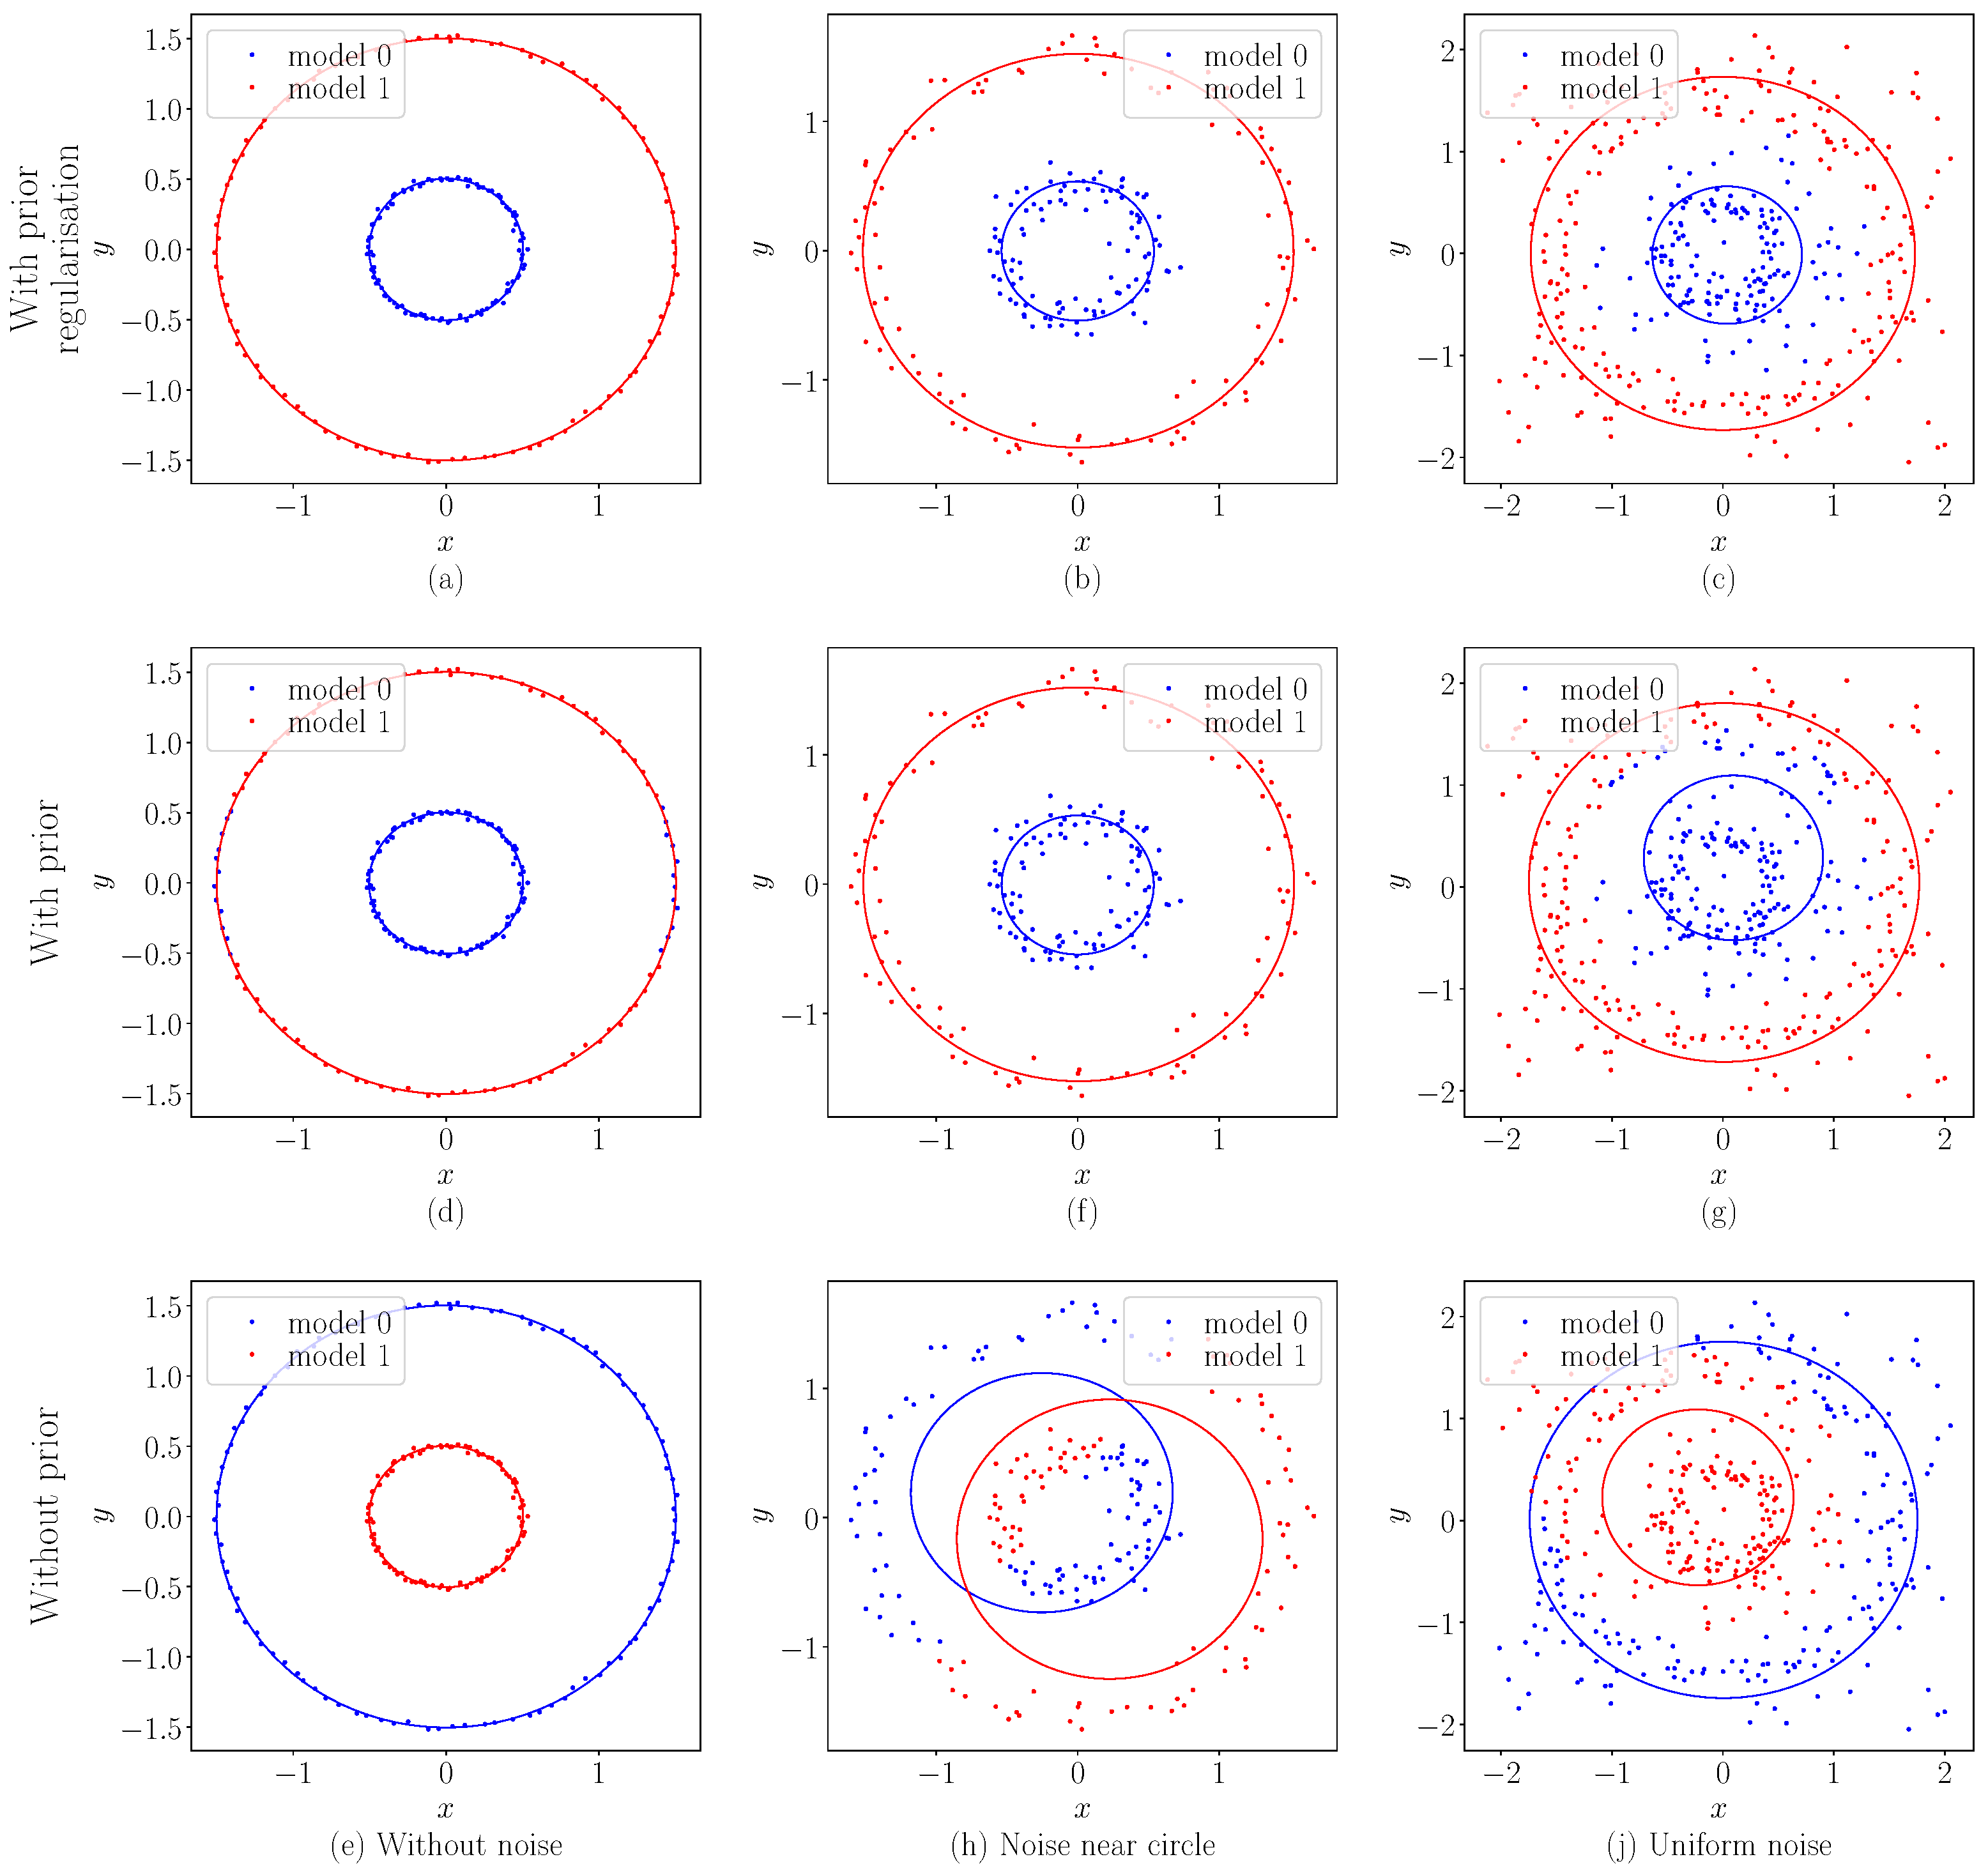
\includegraphics[width=1\textwidth]{result_eng/experiment_synthetic}
\caption{A multimodel depending on different prior distribution and depending on different noise levels: (a)--(c) multimodel with prior regularization; (d)--(g) multimodel with simple prior; (e)--(j) multimodel without any priors.}
\label{experiment:1}
\end{figure}
The computational experiment compares quality of mixture of experts~$\mathfrak{M}_1, \mathfrak{M}_2, \mathfrak{M}_3$ on the synthetic dataset.

Synthetic data was generated as two concentric circles with different noise levels.
The Synthetic~1 is the image without any noises, the Synthetic~2 is the image with a noise radius and the Synthetic~3 is an image with uniform noise.

The fig.~\ref{experiment:1} shows results of multimodels~$\mathfrak{M}_1, \mathfrak{M}_2, \mathfrak{M}_3$.
All multimodels did 50 iterations of the EM-algorithm.
Multimodels~$\mathfrak{M}_2, \mathfrak{M}_3$ approximate circles better than multimodel~$\mathfrak{M}_1$. The tab.~\ref{tb:ce:1} shows the approximation quality~\eqref{eq:ce:ex:0:1} for all multimodels.

\begin{table}[h!t]
\begin{center}
\caption{The approximation quality~\eqref{eq:ce:ex:0:1} for all multimodels}
\label{tb:ce:1}
\begin{tabular}{|c|c|c|c|}
\hline
	Dataset & $\mathcal{S}_{\mathfrak{M}_1}$ & $\mathcal{S}_{\mathfrak{M}_2} $& $\mathcal{S}_{\mathfrak{M}_3} $\\
	\hline
	\multicolumn{1}{|l|}{Synthetic~1}
	& $10^{-5}$& $10^{-5}$& $10^{-5}$\\
	\hline
	\multicolumn{1}{|l|}{Synthetic~2}
	& $0.6$& $10^{-3}$& $10^{-3}$\\
	\hline
	\multicolumn{1}{|l|}{Synthetic~3}
	& $0.6$& $10^{-3}$& $10^{-3}$\\
\hline
\end{tabular}
\end{center}
\end{table}

\paragraph{Learning process on synthetic data.}
\begin{figure}[h!t]\center
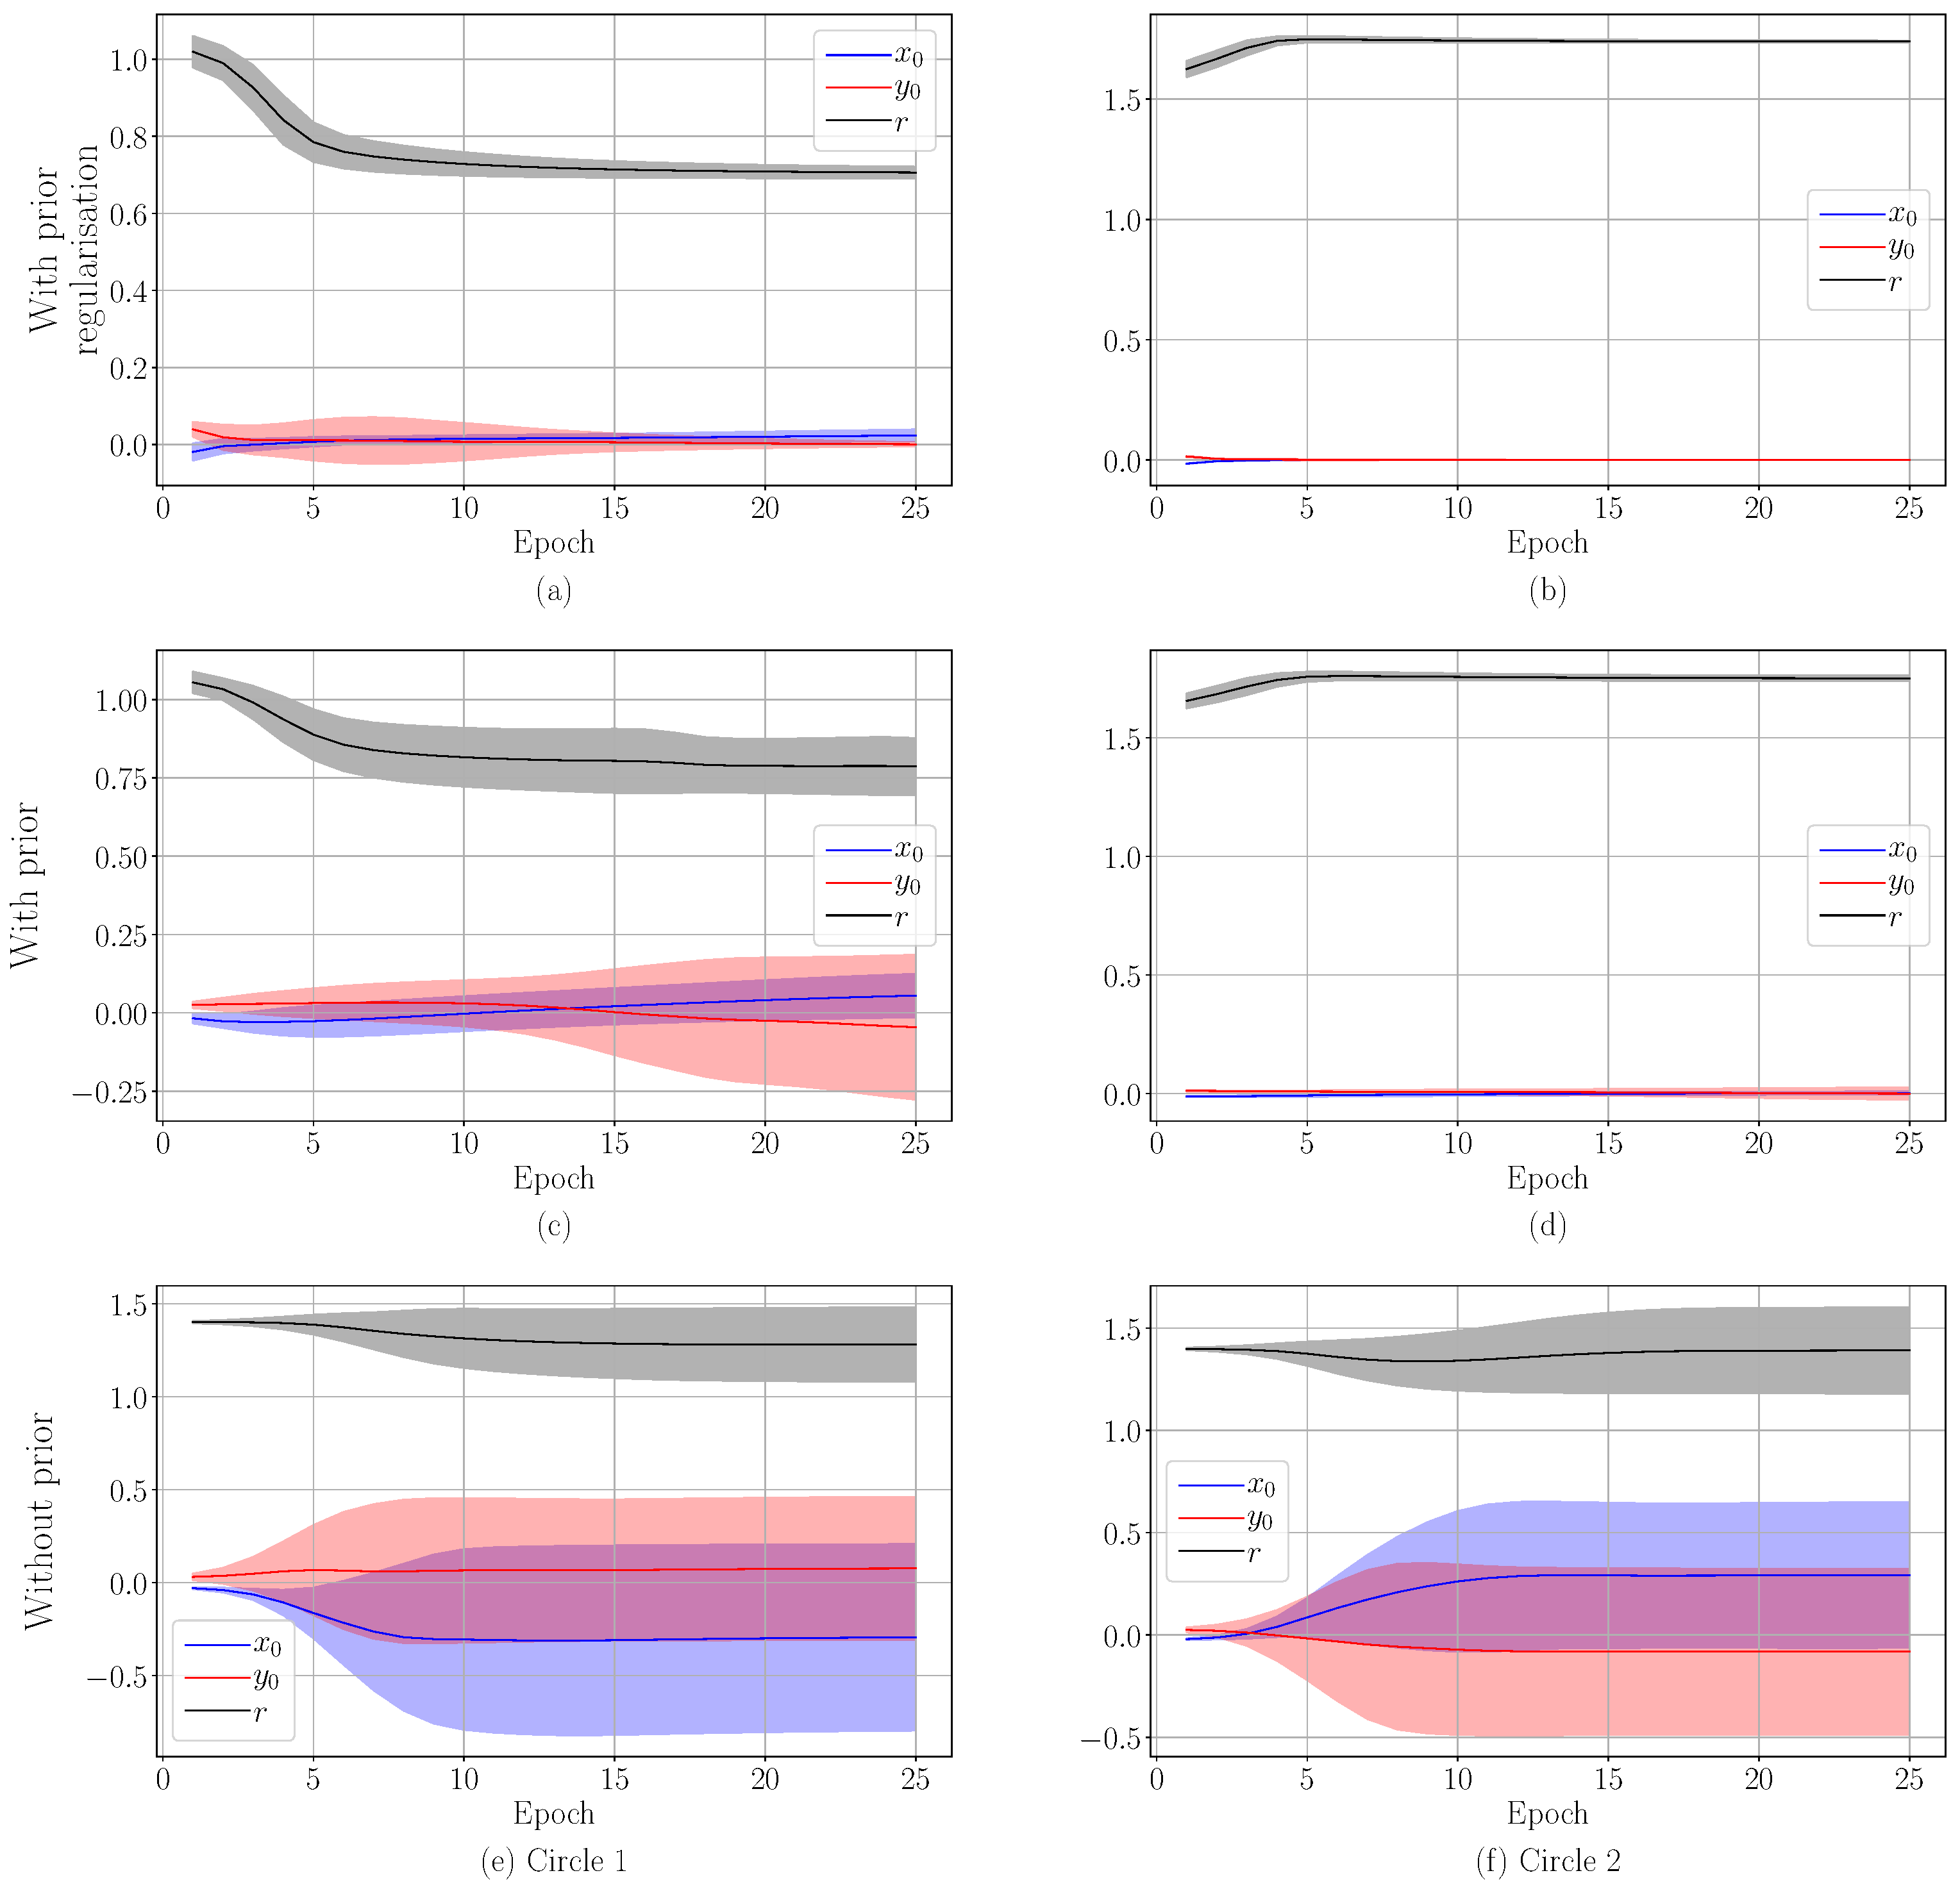
\includegraphics[width=1\textwidth]{result_eng/experiment_synthetic_param_progress}
\caption{The dependence of center and radius on the iteration number: (a)--(b) multimodel with prior regularization; (e)--(d) multimodel with simple prior; (e)--(f) multimodel without any priors.}
\label{experiment:st:2:1}
\end{figure}

\begin{figure}[h!t]\center
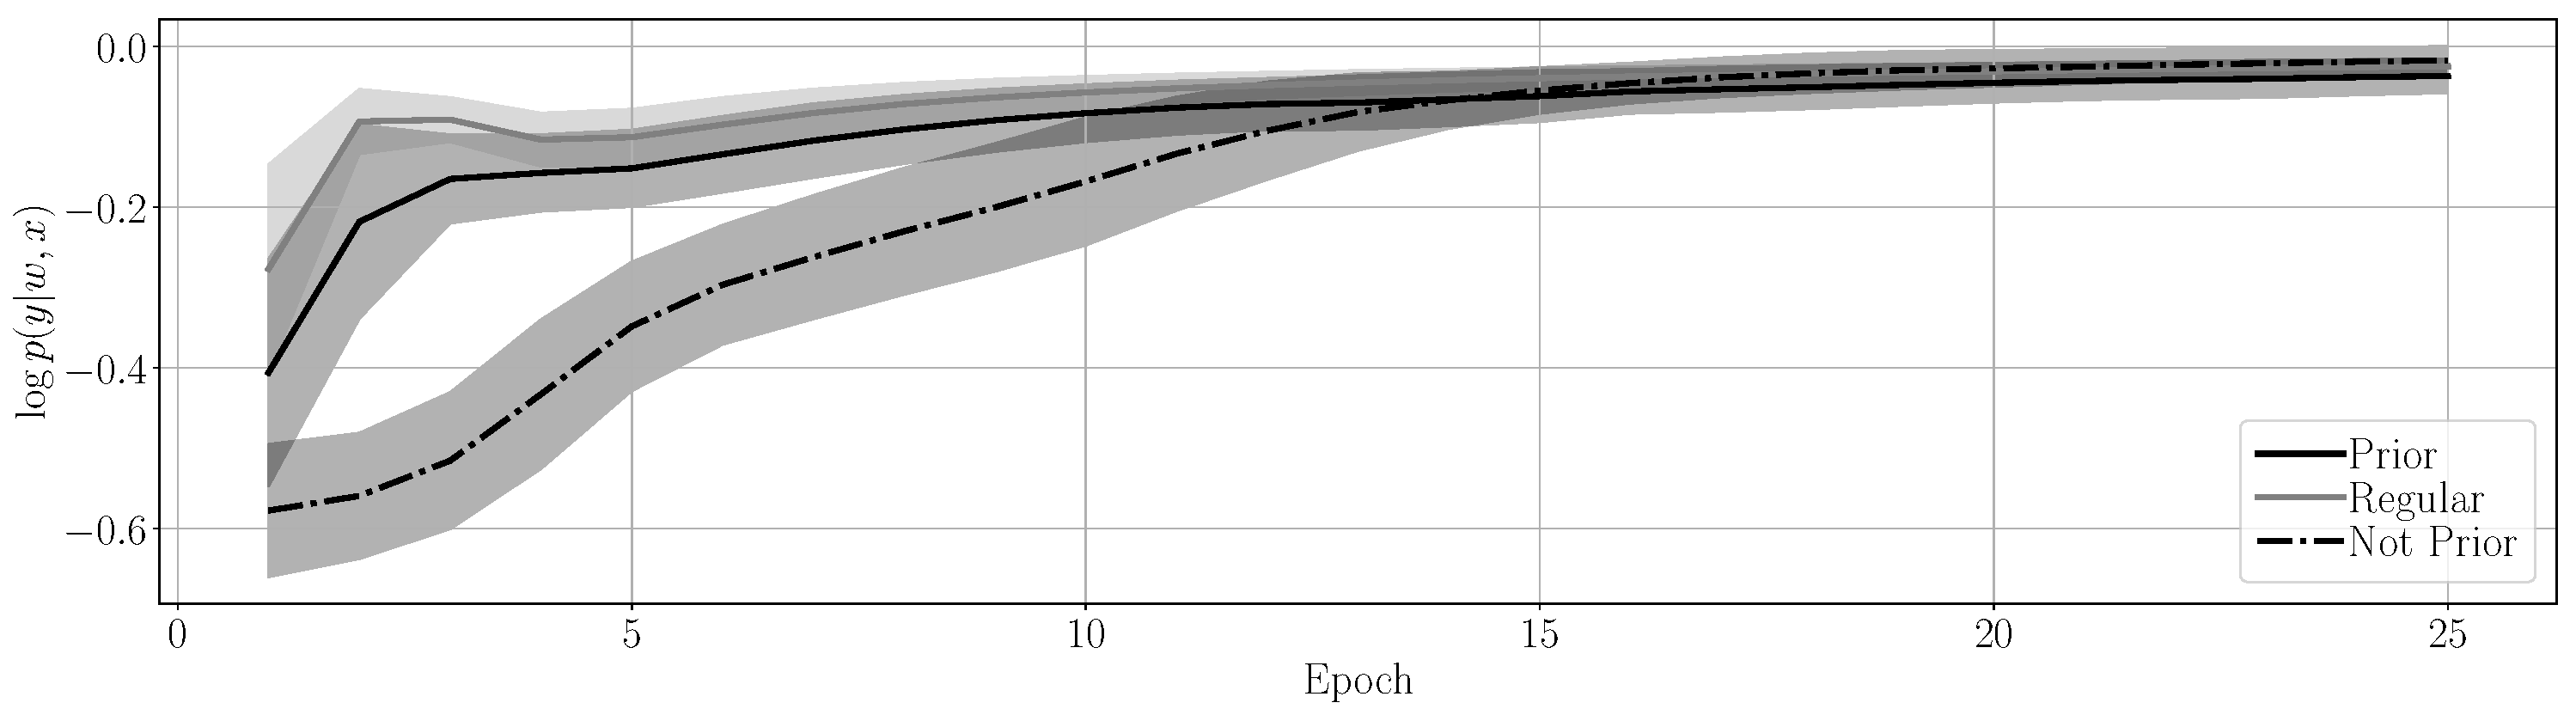
\includegraphics[width=1\textwidth]{result_eng/experiment_synt_likelihood_progress}
\caption{The dependence of log-likelihood~\eqref{eq:ce:st:2:1} on the iteration number.}
\label{experiment:st:2:2}
\end{figure}

\begin{figure}[h!t]\center
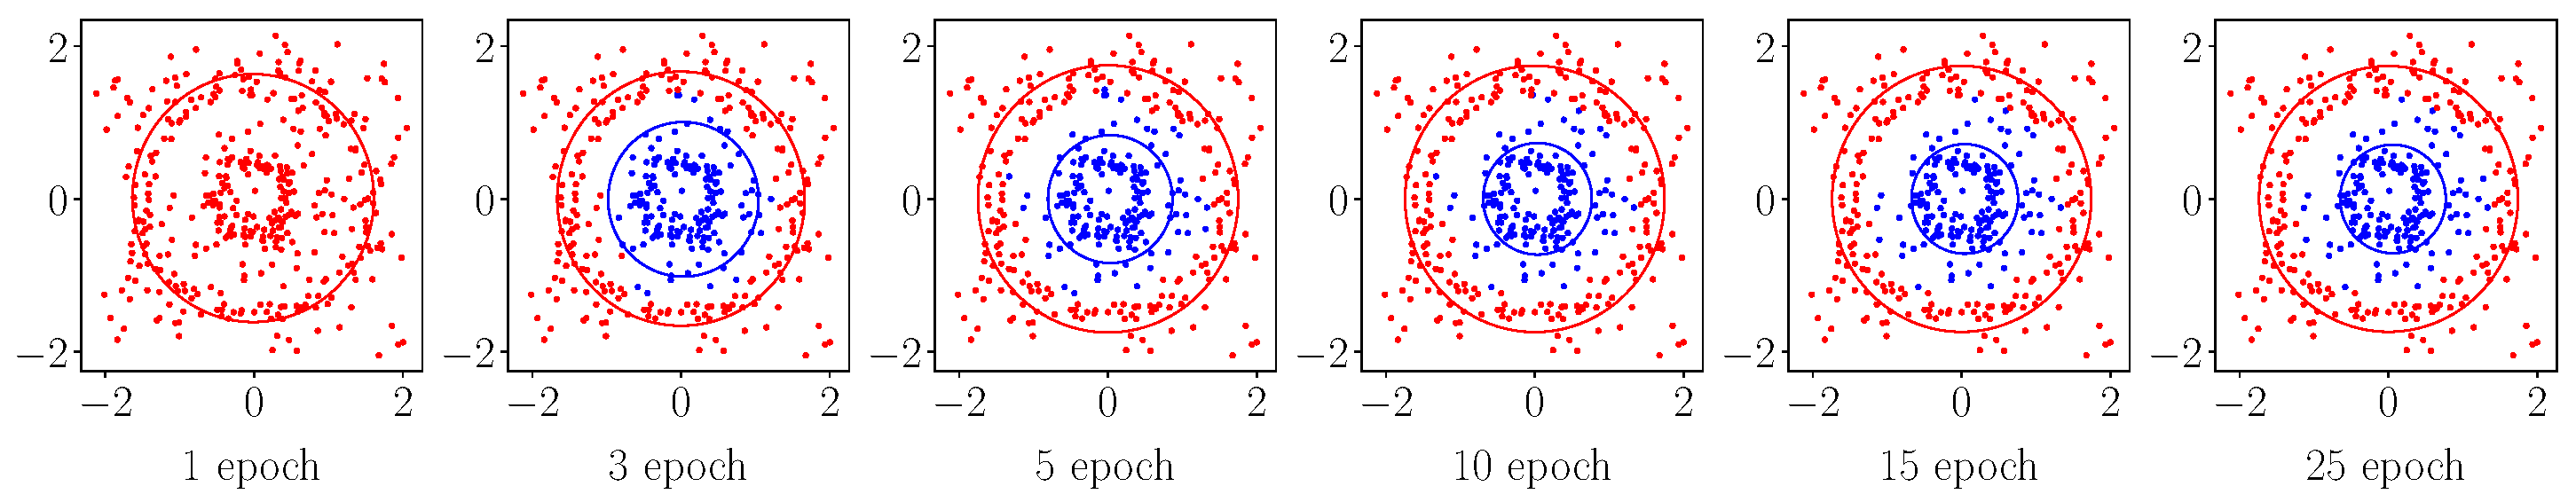
\includegraphics[width=1\textwidth]{result_eng/experiment_synt_regular_progress}
\caption{Learning process visualisation for the multimodel with prior regularisation.}
\label{experiment:st:2:3}
\end{figure}

\begin{figure}[h!t]\center
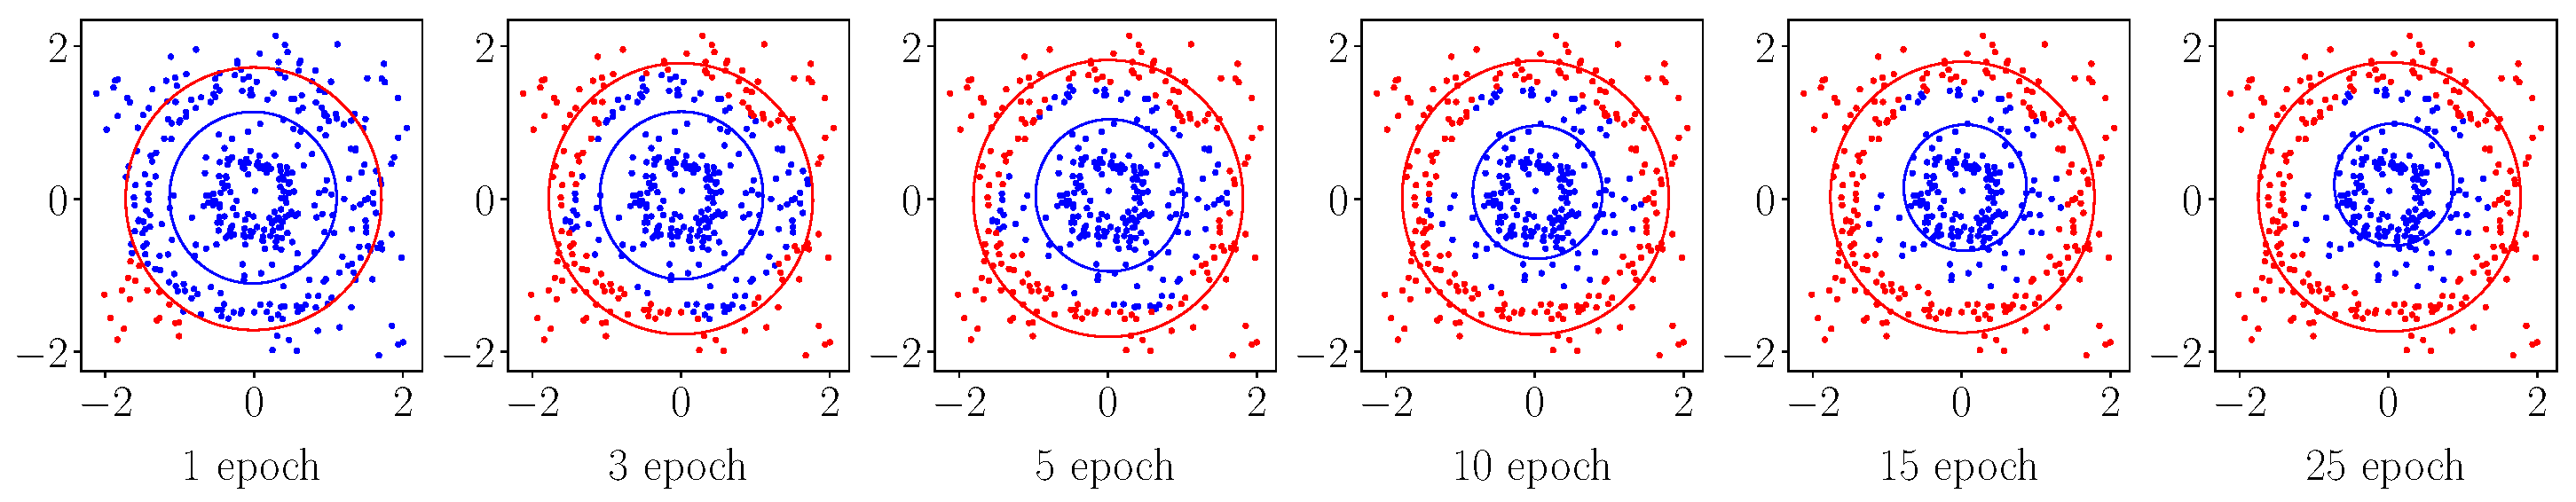
\includegraphics[width=1\textwidth]{result_eng/experiment_synt_prior_progress}
\caption{Learning process visualisation for the multimodel with simple prior.}
\label{experiment:st:2:4}
\end{figure}

\begin{figure}[h!t]\center
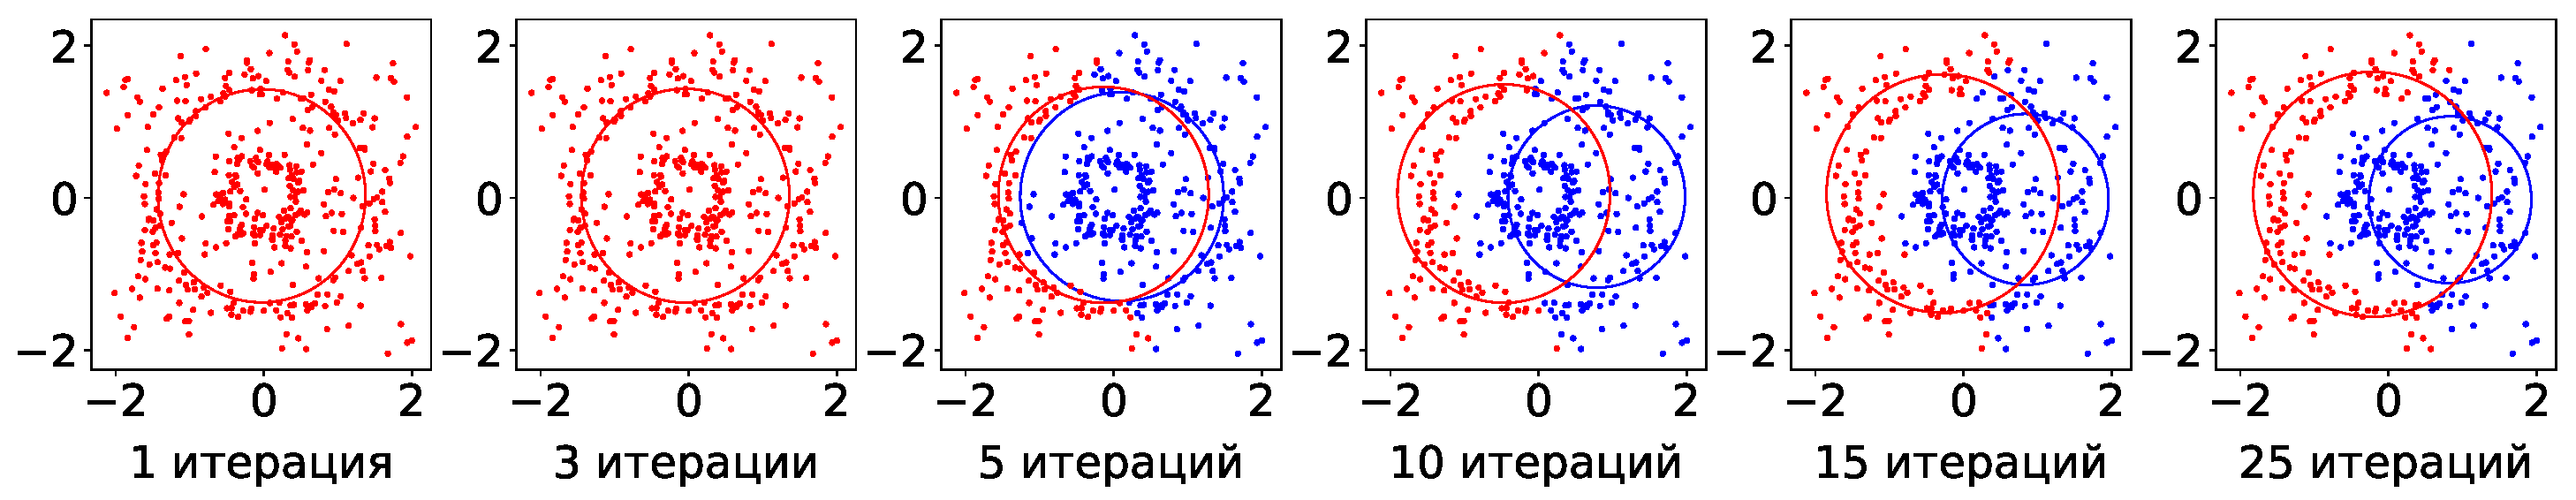
\includegraphics[width=1\textwidth]{result_eng/experiment_synt_not_prior_progress}
\caption{Learning process visualisation for the multimodel without any priors.}
\label{experiment:st:2:5}
\end{figure}
The experiment analyzes multimodels~$\mathfrak{M}_1, \mathfrak{M}_2, \mathfrak{M}_3$ during the EM-algorithm convergence. Multimodels were analysed on the synthetic dataset~Synthetic~3.

The fig.~\ref{experiment:st:2:1} shows the dependence of the radius and center on the EM-algorithm iteration number.
The multimodel with prior distribution for the parameters~$\mathfrak{M}_2$  approximates circles better than multimodel~$\mathfrak{M}_1$ without any priors.
The multimodel with prior regularisation~$\mathfrak{M}_3$ approximates circles more stable than multimodel~$\mathfrak{M}_2$.

The fig.~\ref{experiment:st:2:2} shows the dependence of log-likelihood~\eqref{eq:ce:st:2:1} on the EM-algorithm iteration number.
The log-likelihood of multimodels~$\mathfrak{M}_2, \mathfrak{M}_3$ is growing faster than multimodel~$\mathfrak{M}_1$.  After the 20th iteration all three multimodels have the same log-likelihood.

The fig.~\ref{experiment:st:2:3}-\ref{experiment:st:2:5} show learning process for multimodels~$\mathfrak{M}_1, \mathfrak{M}_2, \mathfrak{M}_3$.
The fig.~\ref{experiment:st:2:5} shows multimodel~$\mathfrak{M}_1$, which does not approximate circles correctly.
The fig.~\ref{experiment:st:2:3}-\ref{experiment:st:2:4} show multimodels~$\mathfrak{M}_2, \mathfrak{M}_3$, which approximate circles correctly.

The experiment shows that multimodels~$\mathfrak{M}_2, \mathfrak{M}_3$ with prior distribution for the parameters approximate circles better than multimodel~$\mathfrak{M}_1$ without any priors.


\paragraph{Multimodels analysis depending on the noise level.} 
\begin{figure}[h!t]\center
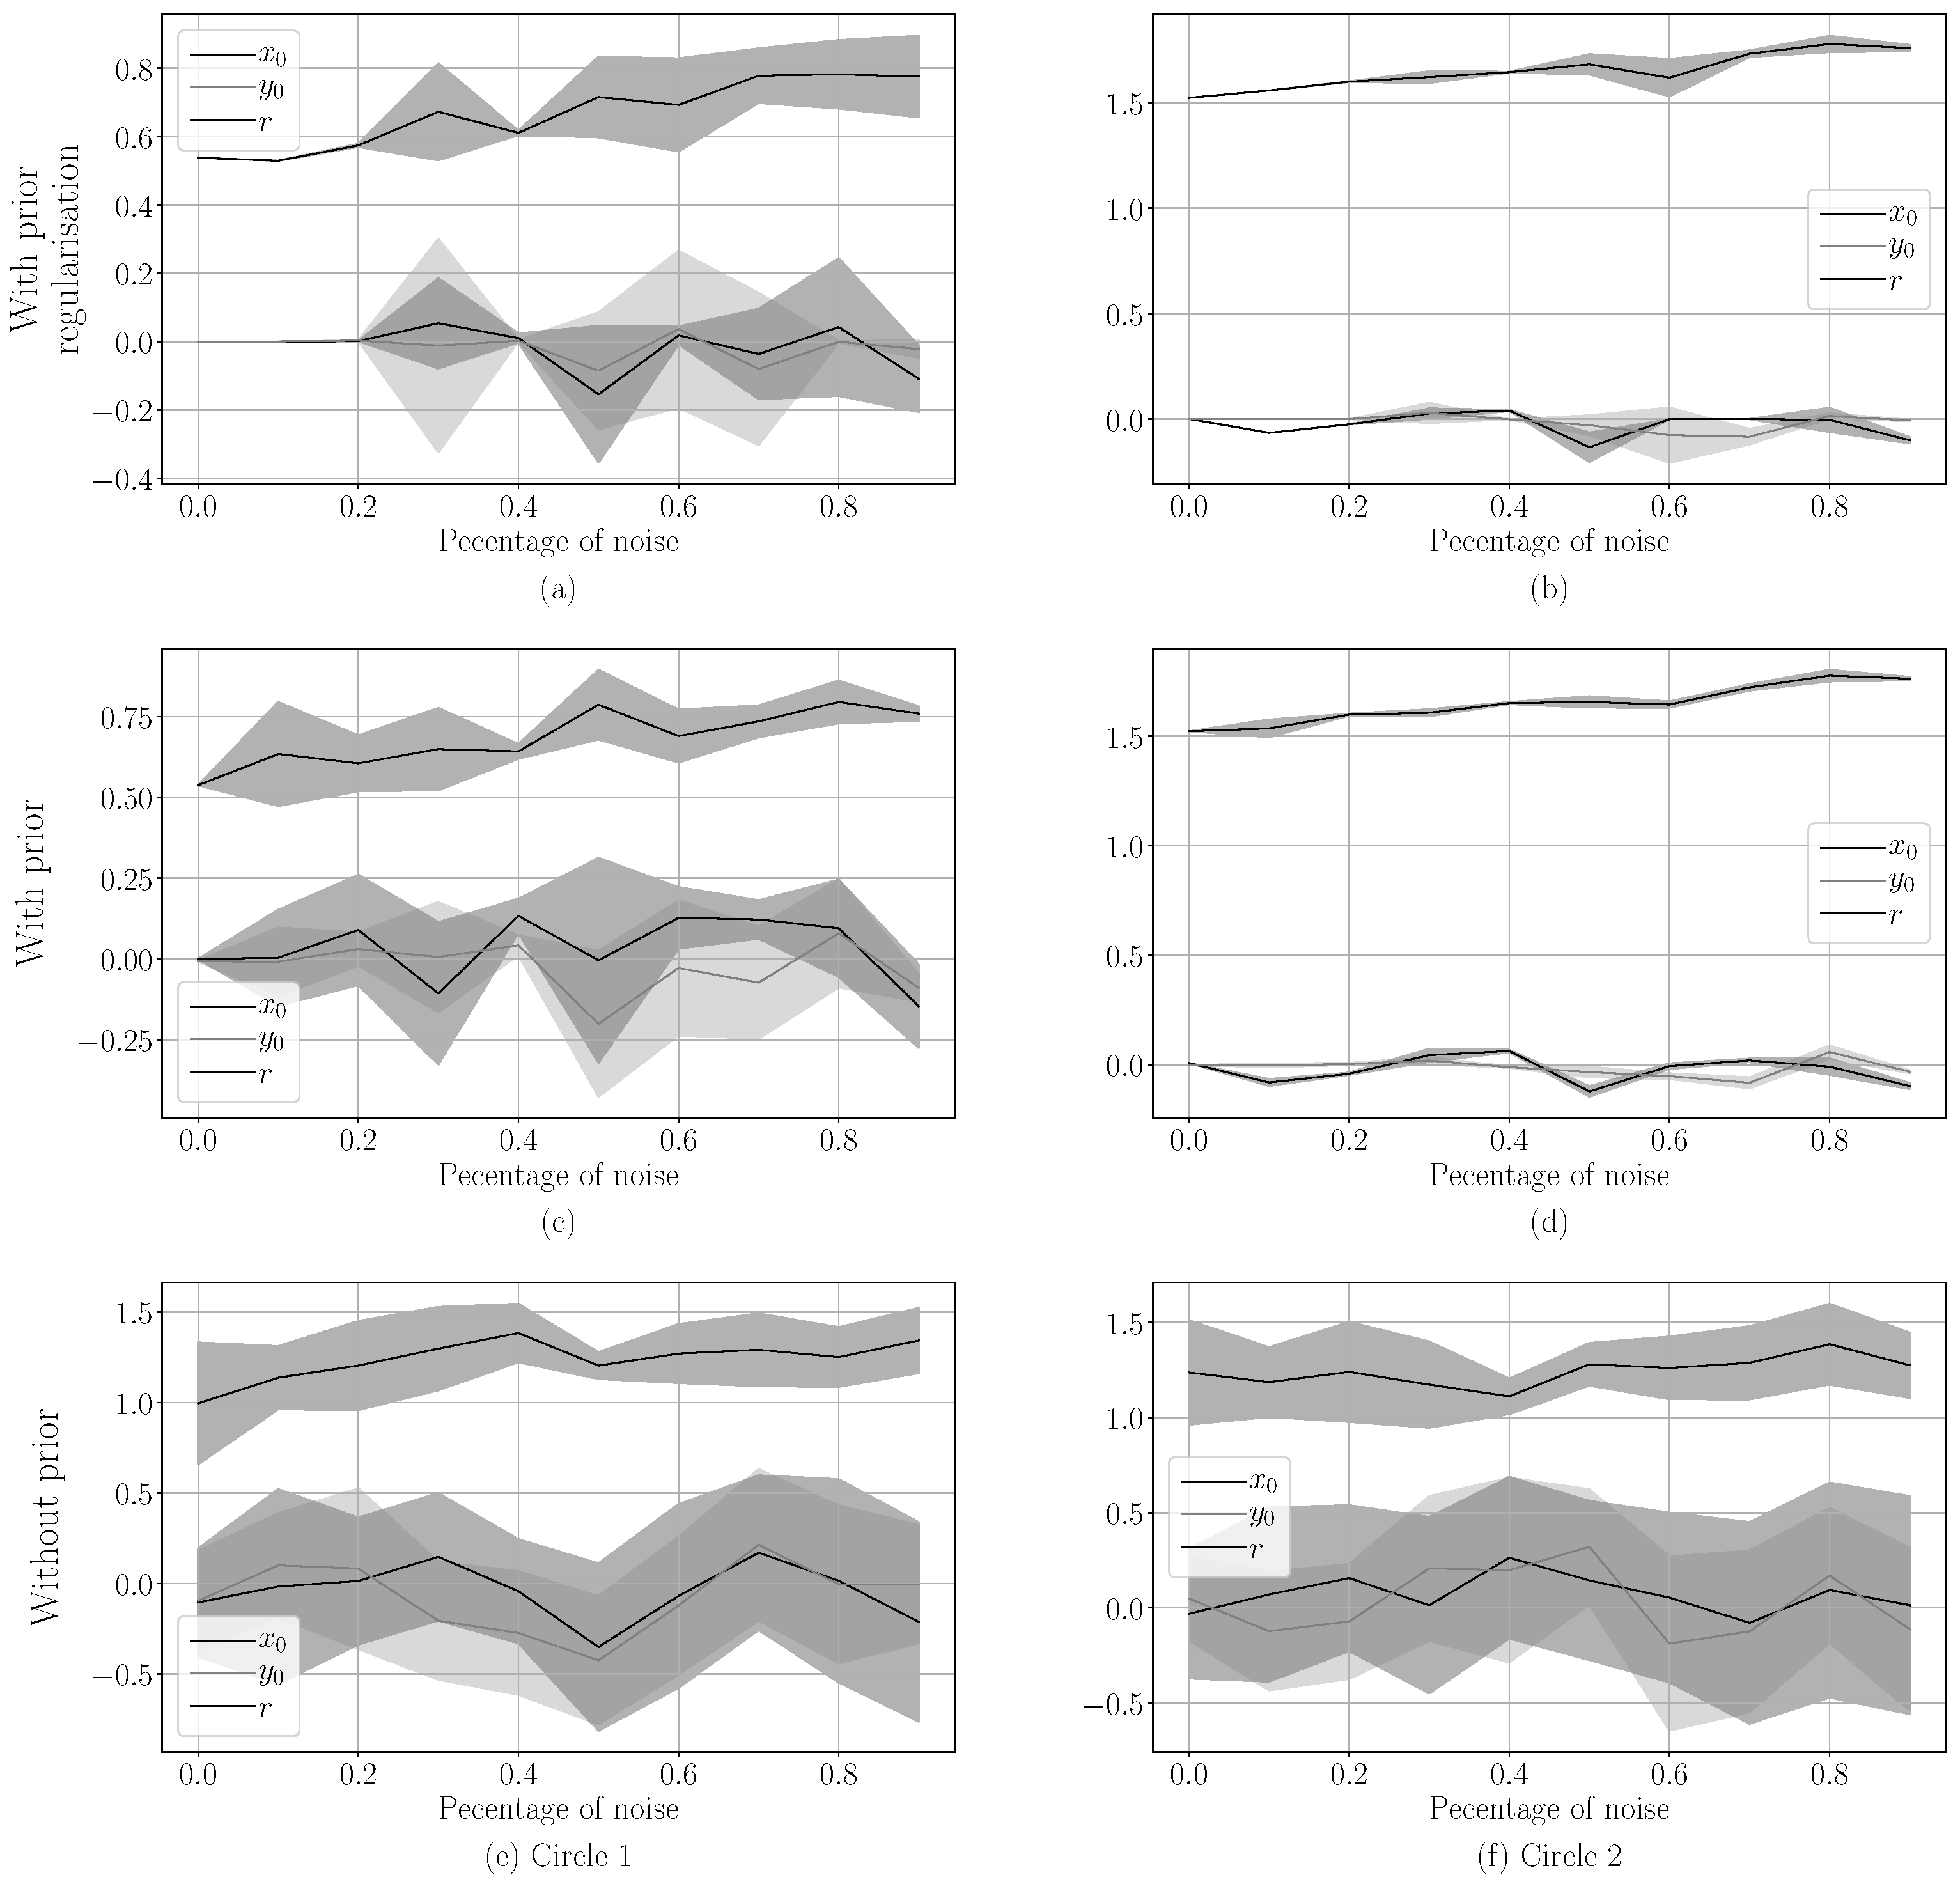
\includegraphics[width=1\textwidth]{result_eng/experiment_synthetic_param_progress_noise}
\caption{The dependence of center and radius on the noise level: (a)--(b) multimodel with prior regularization; (c)--(d) multimodel with simple prior; (e)--(f) multimodel without any priors.}
\label{experiment:st:3:1}
\end{figure}

\begin{figure}[h!t]\center
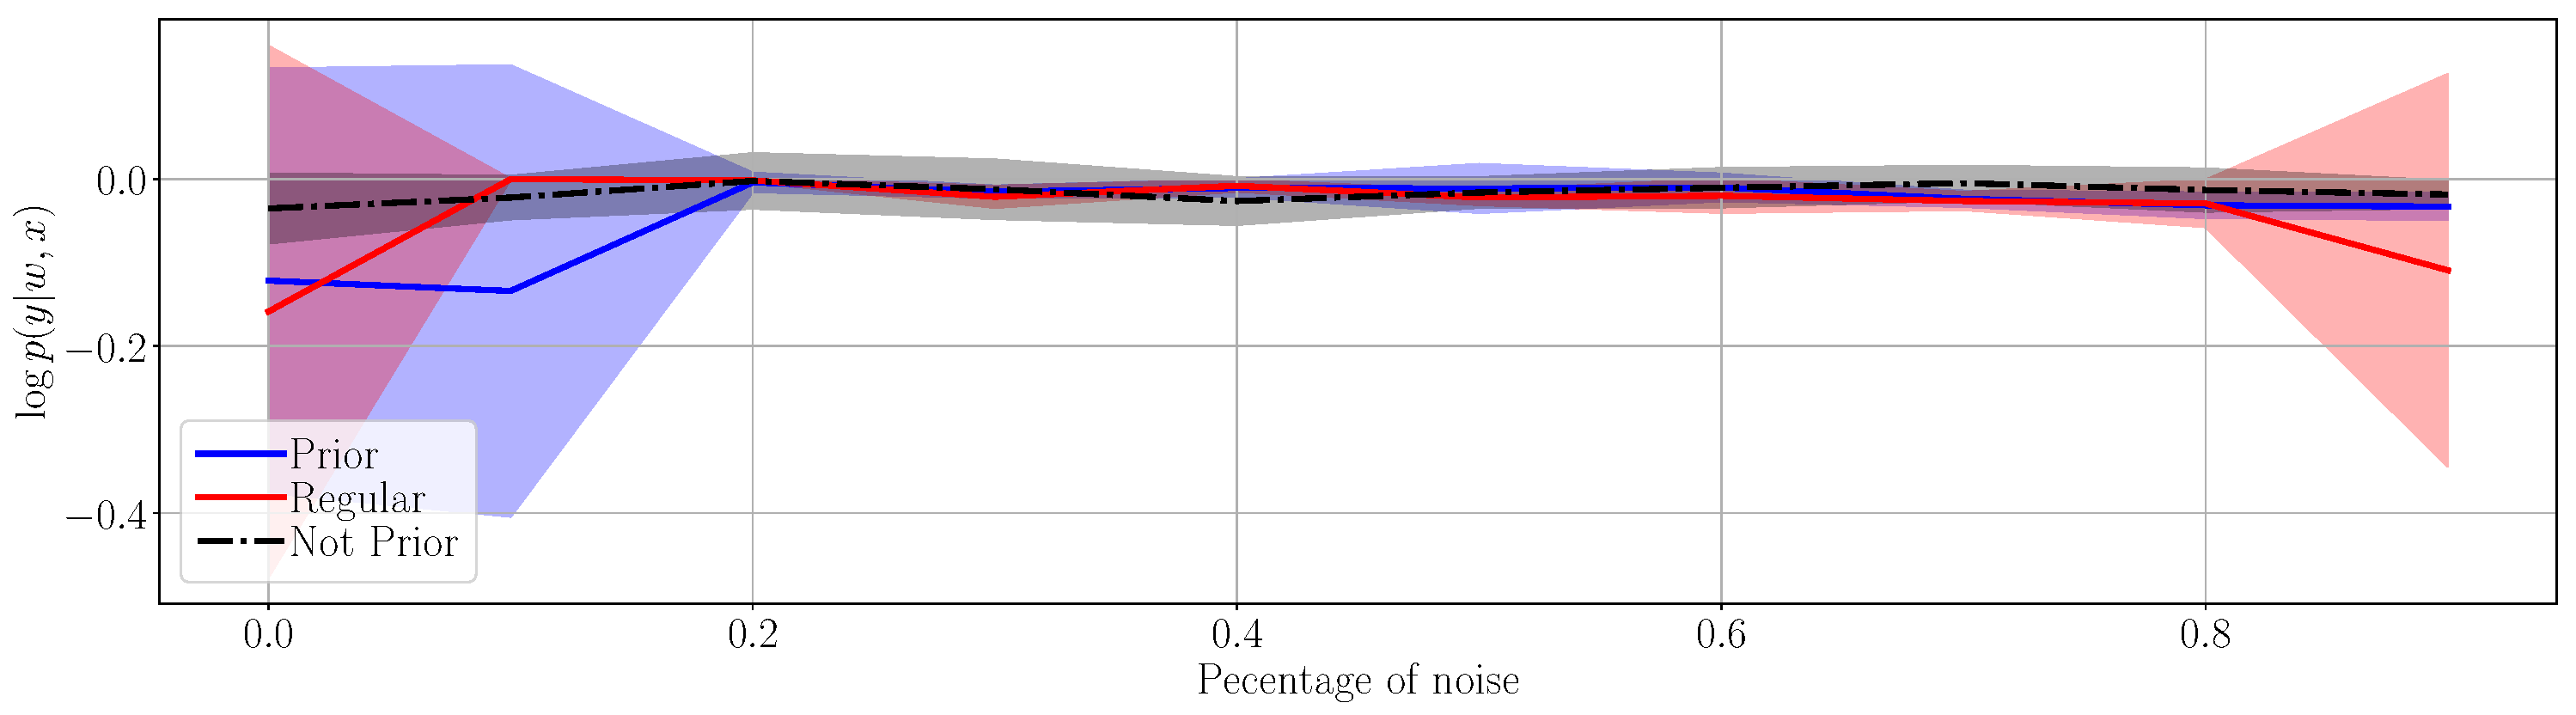
\includegraphics[width=1\textwidth]{result_eng/experiment_synt_likelihood_progress_noise}
\caption{The dependence of log-likelihood~\eqref{eq:ce:st:2:1} on the noise level.}
\label{experiment:st:3:2}
\end{figure}

The experiment analyzes dependence of multimodels~$\mathfrak{M}_1, \mathfrak{M}_2, \mathfrak{M}_3$ on the noise level. 
Multimodels were analysed on the synthetic dataset~Synthetic~1, with adding various noise level.
The lowest noise level is equal to $0$, when no noise. The highest noise level is equal to $1$, when number of noise datum is equal to number of point in circles.

The fig.~\ref{experiment:st:3:1} shows the dependence of center and radius on the noise level. It shows that circle radius increases with increasing noise level. 
The multimodels~$\mathfrak{M}_2, \mathfrak{M}_3$ approximate circles center correctly, but the multimodel~$ \mathfrak{M}_3$ is more stable.

The fig.~\ref{experiment:st:3:2} shows the dependence of log-likelihood~\eqref{eq:ce:st:2:1} on the noise level. 
It shows that log-likelihood~\eqref{eq:ce:st:2:1} is the same for all multimodels, but the fig.~\ref{experiment:st:3:1} shows that the approximation quality~\eqref{eq:ce:ex:0:1} depends on multimodels.

This part of the experiment shows that multimodel~$\mathfrak{M}_3$ with prior regularisation is the most stable model.

\paragraph{Real data.}
\begin{figure}[h!t]\center
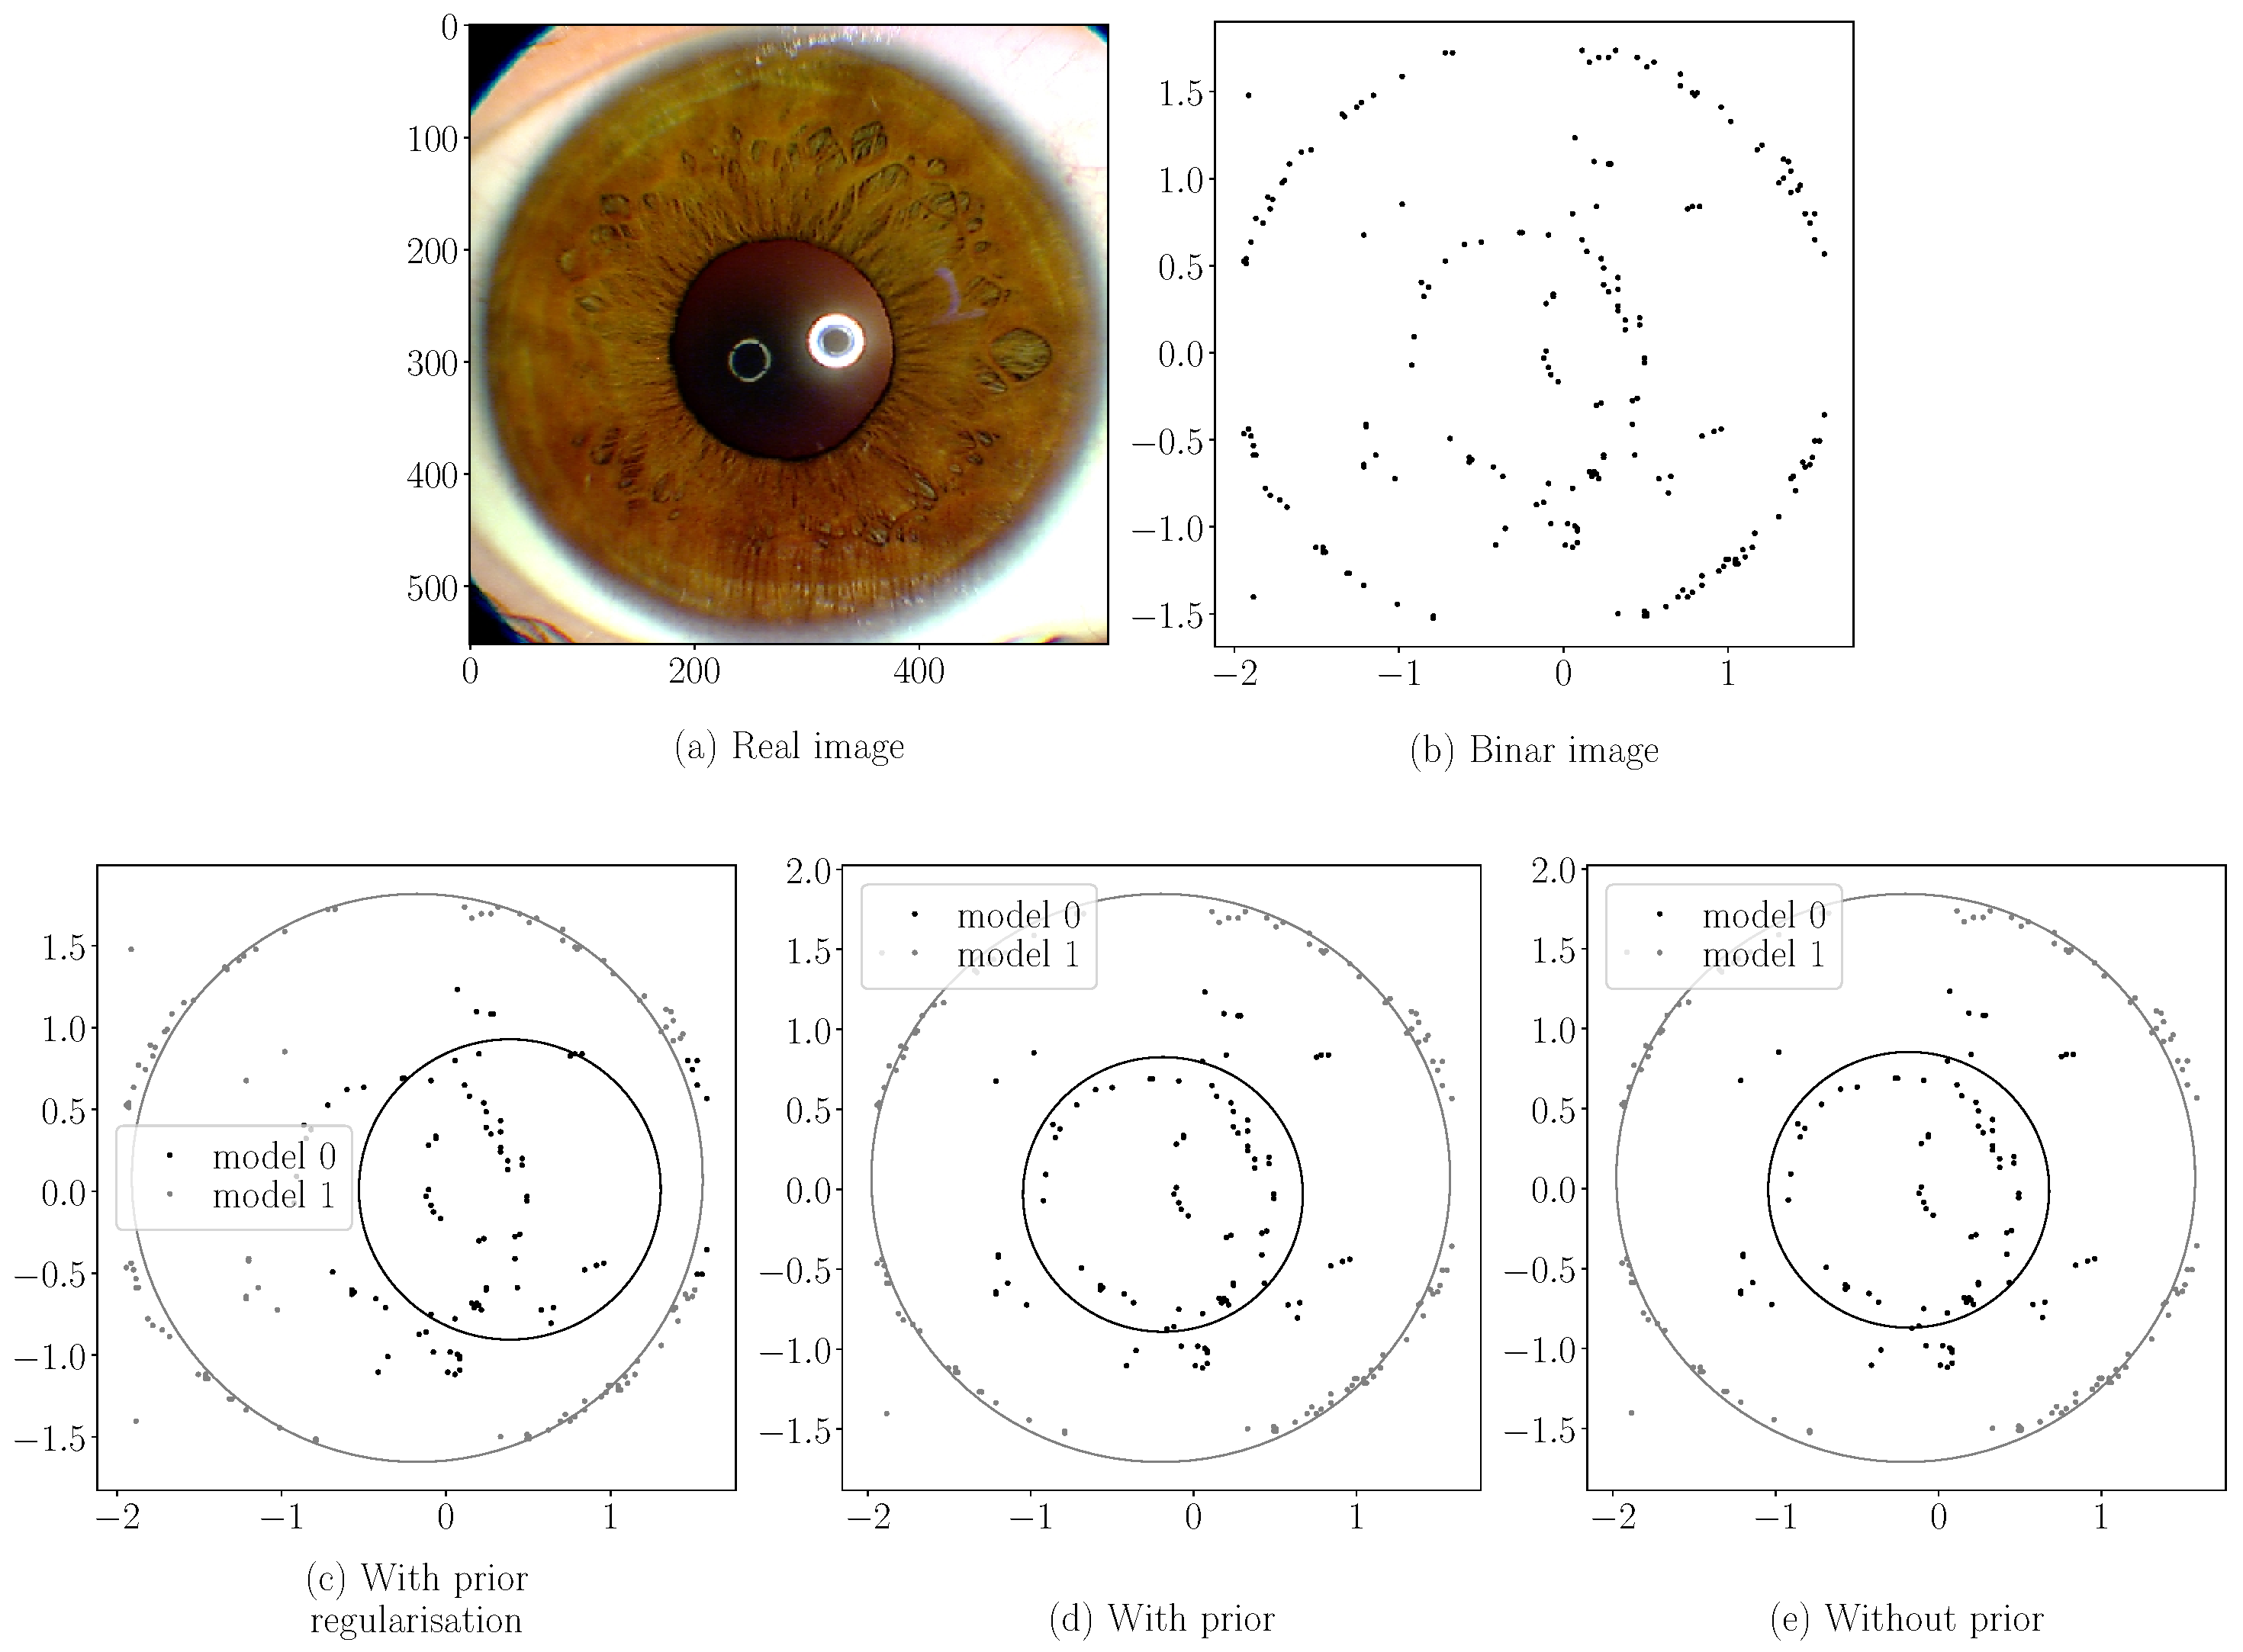
\includegraphics[width=0.9\textwidth]{result_eng/experiment_real_compare}
\caption{Different multimodels on the real image: (a) source image; (b) binarize image; (c) multimodel without any priors; (d) multimodel with simple prior; (e) multimodel with prior regularisation.}
\label{experiment:2}
\end{figure}

This part of the experiment analyzes multimodels~$\mathfrak{M}_1, \mathfrak{M}_2, \mathfrak{M}_3$ on the real data.

The fig.~\ref{experiment:2} shows the result of different multimodels.
The multimodel~$\mathfrak{M}_1$ approximates incorrectly one of the circles.
The multimodels~$\mathfrak{M}_2, \mathfrak{M}_3$ approximate both circles correctly.

\begin{figure}[h!t]\center
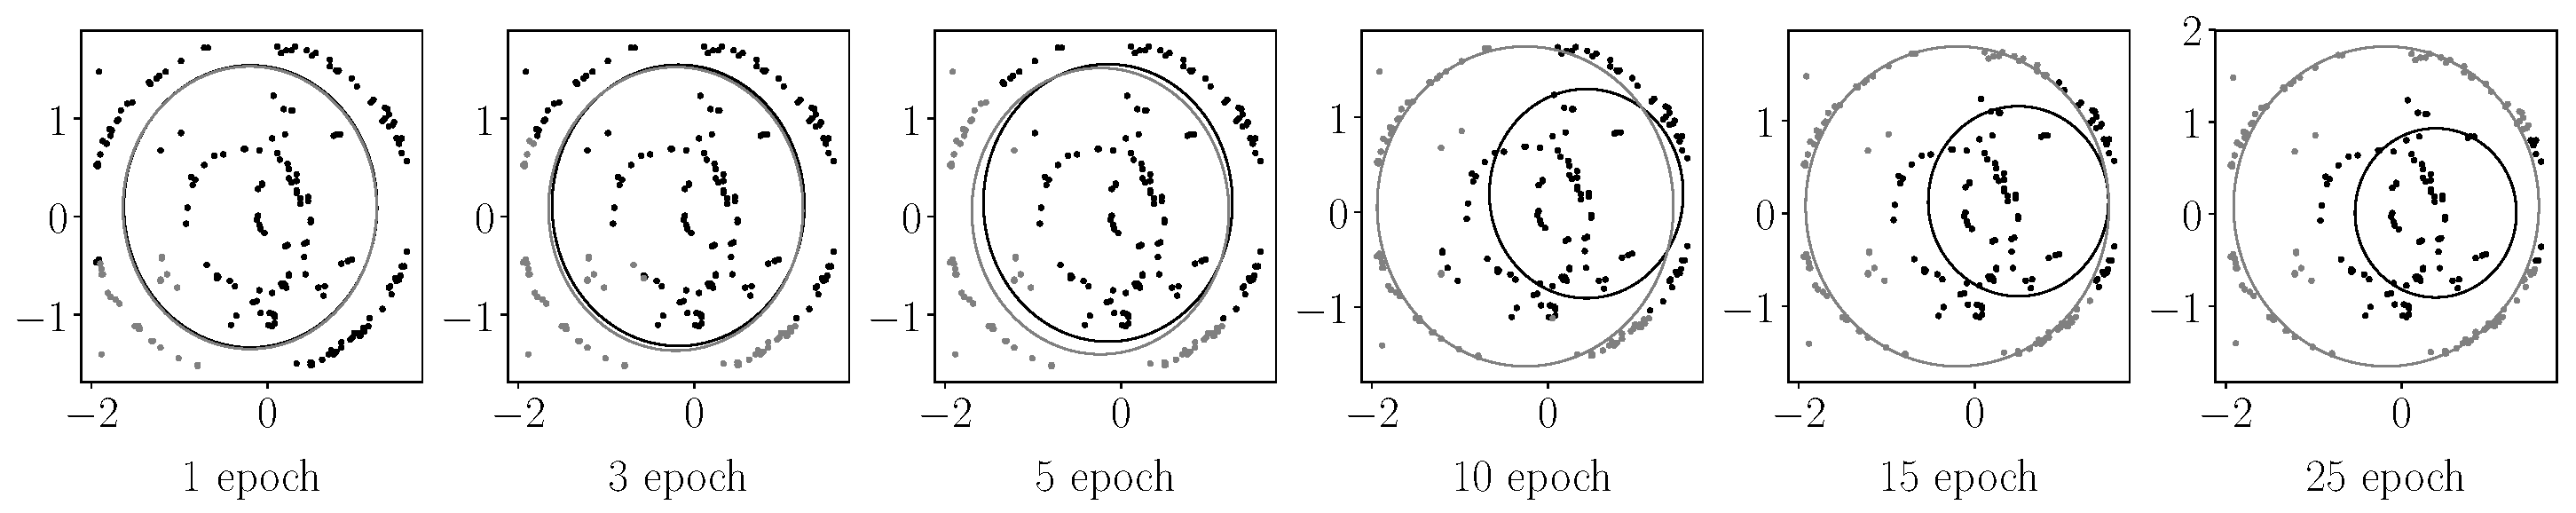
\includegraphics[width=1\textwidth]{result_eng/experiment_real_not_prior}
\caption{Learning process visualisation for the multimodel without any priors.}
\label{experiment:3}
\end{figure}

\begin{figure}[h!t]\center
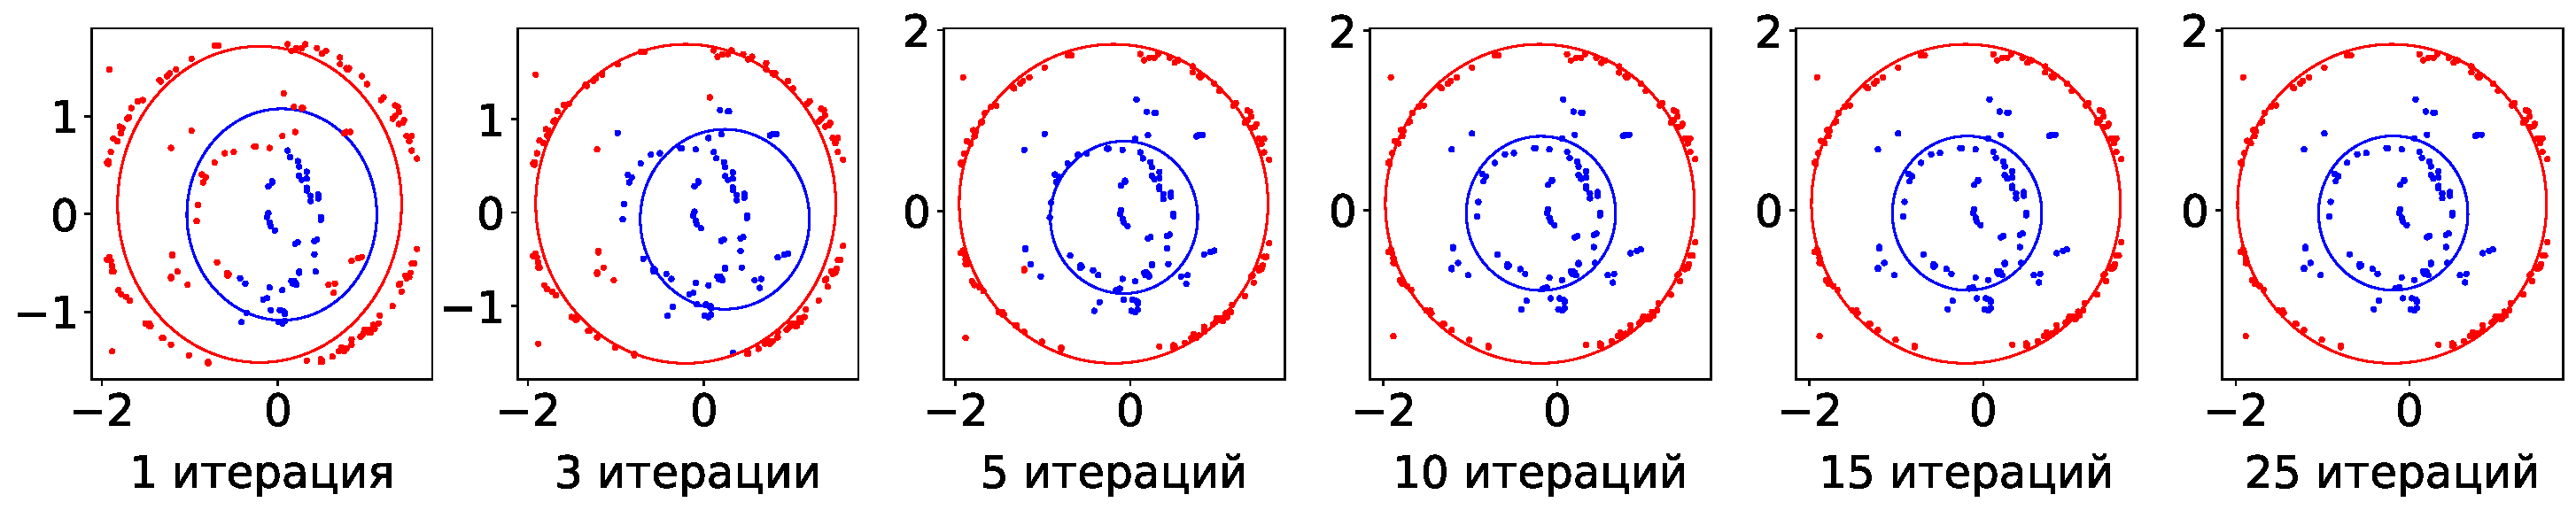
\includegraphics[width=1\textwidth]{result_eng/experiment_real_prior}
\caption{Learning process visualisation for the multimodel with simple prior.}
\label{experiment:4}
\end{figure}

\begin{figure}[h!t]\center
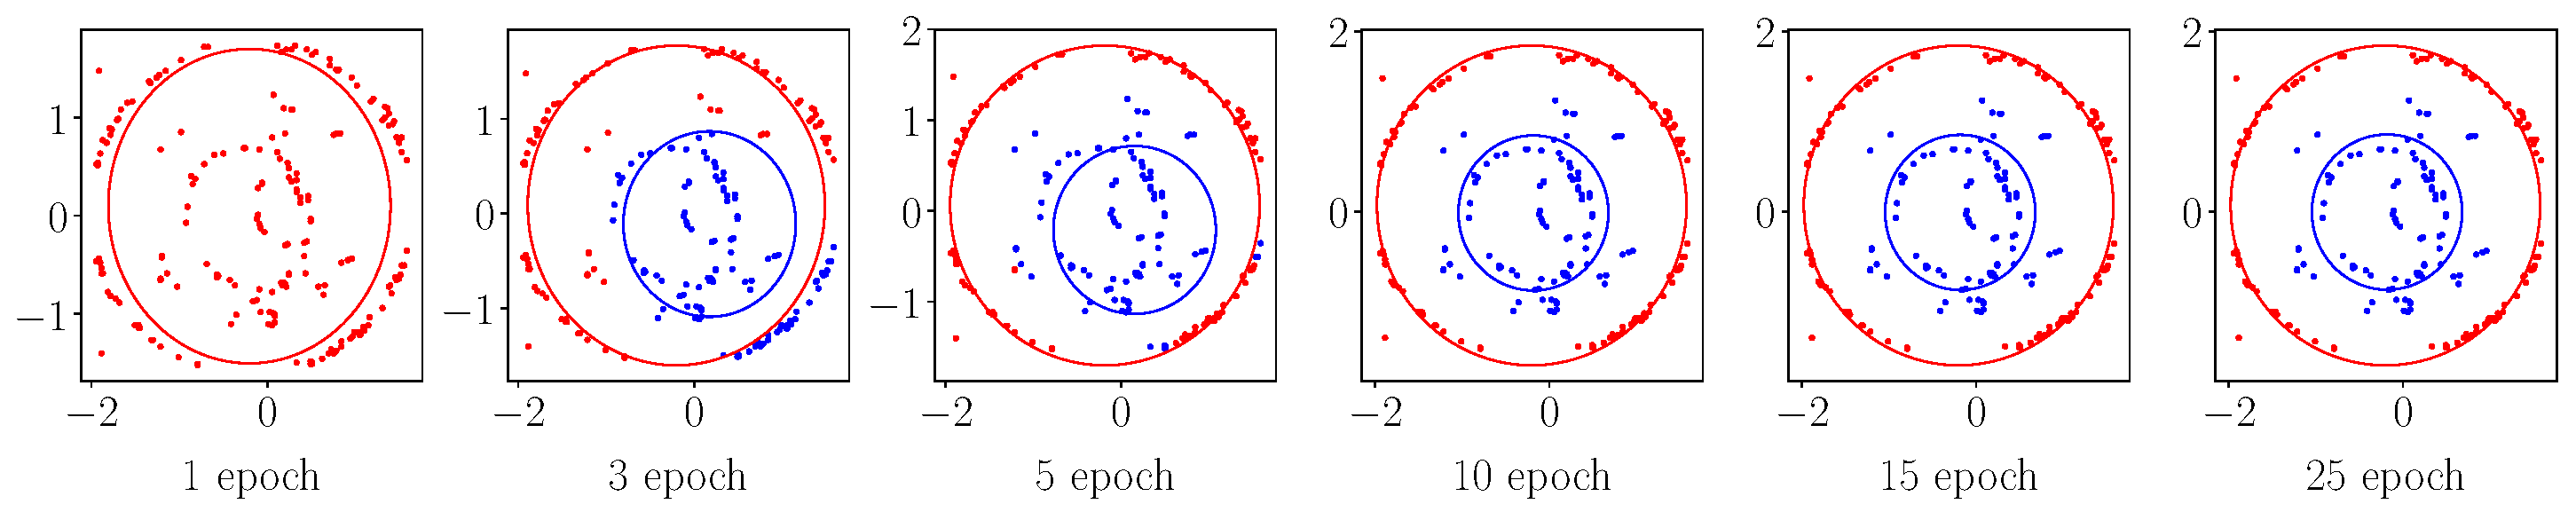
\includegraphics[width=1\textwidth]{result_eng/experiment_real_regular}
\caption{Learning process visualisation for the multimodel with prior regularisation.}
\label{experiment:5}
\end{figure}

The fig.~\ref{experiment:3}-\ref{experiment:5} show learning process for multimodels~$\mathfrak{M}_1, \mathfrak{M}_2, \mathfrak{M}_3$.
The fig.~\ref{experiment:3} shows multimodel~$\mathfrak{M}_1$.
The fig.~\ref{experiment:4} shows multimodel~$\mathfrak{M}_2$.
The fig.~\ref{experimen:5} shows multimodel~$\mathfrak{M}_3$.

This part of experiment shows that multimodels~$\mathfrak{M}_2, \mathfrak{M}_3$ approximate circles better than multimodel~$\mathfrak{M}_1$ even for the real images.


\section{Conclusion}
The paper compares multimodels with different prior distributions for the model parameters. Concentric circles with different noises are data in a computational experiment. Linear models were used to approximate the circles in the image. The gate function is a two-layer fully connected neural network.

The experiment compares the model with the prior distribution and without it. The multimodel with prior distribution is more accurate compared to the model without prior distribution.

Another experiment compares different types of regularization. The experiment showed that multimodel with regularization is more stable.

The experiment shows that all models in this article are sensitive to outburst. To solve this problem, it is proposed to use a local model that approximates noise.

In future work, it is planned to improve the multimodel by adding a prior distribution for the gate function parameters. It is planned to add a local model that approximates noise in the data. It is assumed that the probability of noise is low.

\begin{thebibliography}{99}
\bibitem{Tianqi2016}
	\textit{Chen Tianqi, Guestrin Carlos} XGBoost: A Scalable Tree Boosting System~// KDD ’16 Proceedings of the 22nd ACM SIGKDD International Conference on Knowledge Discovery and Data Mining. 2016.
	
\bibitem{Ishwaran2012}
	\textit{Chen Xi, Ishwaran Hemant} Random Forests for Genomic Data Analysis~// Genomics. 2012. Issues. 99, No 6. pp. 323--329.

\bibitem{Yuksel2012}
	\textit{Yuksel Seniha Esen, Wilson Joseph N., Gader Paul D} Twenty Years of Mixture of Experts~// IEEE Transactions on Neural Networks and Learning Systems. 2012. Issues. 23, No 8. pp. 1177--1193.

\bibitem{Shazeer2017}
	\textit{Noam Shazeer, Azalia Mirhoseini, Krzysztof Maziarz} Outrageously large neural networks: the sparsely-gated mixture-of-experts layer~// ICLR, 2017.

\bibitem{Edward2002}
	\textit{Rasmussen Carl Edward, Ghahramani Zoubin} Infinite Mixtures of Gaussian Process Experts~// Advances in Neural Information Processing Systems 14. 2002. pp. 881–888.
	
\bibitem{Jordan1994}
	\textit{M.~I.~Jordan} Hierarchical mixtures of experts and the EM algorithm~// Neural Comput., vol. 6, no. 2, pp. 181–214, 1994.
	
\bibitem{Lima2007}
	\textit{C.~A.~M.~Lima, A.~L.~V. Coelho, F.~J.~Von~Zuben} Hybridizing mixtures of experts with support vector machines: Investigation into nonlinear dynamic systems identification~// Inf. Sci., vol. 177, no. 10, pp. 2049–2074, 2007.

\bibitem{Cao2003}
	\textit{L.~Cao} Support vector machines experts for time series forecasting~// Neurocomputing, vol. 51, pp. 321–339, Apr. 2003.

\bibitem{Dempster1977}
	\textit{A. P. Dempster, N. M. Laird and D. B. Rubin} Maximum Likelihood from Incomplete Data via the EM Algorithm~// Journal of the Royal Statistical Society. Series B (Methodological), Vol. 39, No. 1 pp. 1-38, 1977.
	
\bibitem{Jordan1991}
	\textit{M.~I.~Jordan, R.~A.~Jacobs} Hierarchies of adaptive experts~// in Advances in Neural Information Processing Systems. Cambridge, MA: MIT Press, 1991, pp. 985–992.
	
\bibitem{Yumlu2003}
	\textit{M.\,S.~Yumlu, F.\,S.~Gurgen,  N.~Okay} Financial time series prediction using mixture of experts~// in Proc. 18th Int. Symp. Comput. Inf. Sci., 2003, pp. 553--560.
	
\bibitem{Cheung1995}
	\textit{Y.~M.~Cheung, W.~M.~Leung, and L. Xu} Application of mixture of experts model to financial time series forecasting~// in Proc. Int. Conf. Neural Netw. Signal Process., 1995, pp. 1--4.
	
\bibitem{Weigend2000}
	\textit{A. S. Weigend, S. Shi} Predicting daily probability distributions of S\&P500 returns~// J. Forecast., vol. 19, no. 4, pp. 375--392, 2000.
	
\bibitem{Ebrahimpour2009}
	\textit{R. Ebrahimpour, M. R. Moradian, A. Esmkhani, F. M. Jafarlou} Recognition of Persian handwritten digits using characterization loci and mixture of experts~// J. Digital Content Technol. Appl., vol. 3, no. 3, pp. 42–46, 2009.
	
\bibitem{Estabrooks2001}
	\textit{A.~Estabrooks, N.~Japkowicz} A mixture-of-experts framework for text classification~//in Proc. Workshop Comput. Natural Lang. Learn., Assoc. Comput. Linguist., 2001, pp. 1--8.
	
\bibitem{Mossavat2010}
	\textit{S. Mossavat, O. Amft, B. de Vries, P. Petkov, W. Kleijn} A Bayesian hierarchical mixture of experts approach to estimate speech quality~// in Proc. 2nd Int. Workshop Qual. Multimedia Exper., pp. 200--205., 2010

\bibitem{Peng1996}
	\textit{F. Peng, R. A. Jacobs, M. A. Tanner} Bayesian inference in mixtures-of-experts and hierarchical mixtures-of-experts models with an application to speech recognition~// J. Amer. Stat. Assoc., vol. 91, no. 435, pp. 953–960, 1996.
	
\bibitem{Tuerk2001}
	\textit{A. Tuerk} The state based mixture of experts HMM with applications to the recognition of spontaneous speech~// Ph.D. thesis, Dept. Eng., Univ. Cambridge, Cambridge, U.K., 2001.
	
\bibitem{Sminchisescu2007}
	\textit{C. Sminchisescu, A. Kanaujia, and D. Metaxas} B M3 E: Discrimina- tive density propagation for visual tracking~// IEEE Trans. Pattern Anal. Mach. Intell., vol. 29, no. 11, pp. 2030–2044, 2007.

\bibitem{Matveev2010}
	\textit{I. Matveev} Detection of iris in image by interrelated maxima of brightness gradient projections~// Appl.Comput. Math. 9 (2), 252–257, 2010.

\bibitem{Matveev2014}
	\textit{I. Matveev, I. Simonenko}. Detecting precise iris boundaries by circular shortest path method~// Pattern Recognition and Image Analysis. 24. 304-309. 2014.
	
\bibitem{Bowyer2010}
	\textit{K. Bowyer, K. Hollingsworth, P. Flynn} A Survey of Iris Biometrics Research: 2008–2010.
	
\bibitem{bishop2006}
	\textit{Bishop C.} Pattern Recognition and Machine Learning.~---~Berlin: Springer, 2006. 758~p.

 \end{thebibliography}
 
 \appendix

\begin{comment}
\section{Постановка задачи нахождения параметров эллипса}\label{apendix:el}
Задано бинарное изображение:
\[
\label{apendix:el:eq:1}
\begin{aligned}
\textbf{M} \in \{0,1\}^{m_1 \times m_2},
\end{aligned}
\]
где $0$ отвечает черной точке --- изображения, $1$ --- белой точке фона.

По изображению $\textbf{M}$ строится выборка $\textbf{C}$, элементами которой являются координаты~$x_i, y_i$ белых точек на картинке:
\[
\label{apendix:el:eq:2}
\begin{aligned}
\textbf{C} \in  \mathbb{R}^{N \times 2},
\end{aligned}
\]
где $N$ --- число черных точек на изображении $\textbf{M}$.

Обозначим $x_0, y_0$ --- центр эллипса, который требуется найти на бинарном изображении $\textbf{M}$, а $a, b$ его коэффициенты вдоль координат. Элементы выборки $\left(x_i, y_i\right)\in\textbf{C}$ являются геометрическим местом точек, которое заданно уравнением эллипса:
\[
\label{apendix:el:eq:3}
\begin{aligned}
\left(x_i - x_0\right)^{2}+\frac{a^2}{b^2}\left(y_i-y_0\right)^2 = a^2.
\end{aligned}
\]
Раскрыв скобки получим уравнение
\[
\label{apendix:el:eq:4}
\begin{aligned}
\left(2x_0\right)\cdot x_i + \left(\frac{2y_0a^2}{b^2}\right)\cdot y_i + \left(-\frac{a^2}{b^2}\right)y_{i}^{2} + \left(a^2-x_0^2-\frac{a^2}{b^2}y_0^2\right)\cdot1 = x_{i}^2.
\end{aligned}
\]
Получаем задачу линейной регрессии для нахождения параметров окружности:
\[
\label{apendix:el:eq:5}
\begin{aligned}
\textbf{X}\textbf{w} \approx \textbf{y},  \quad \textbf{X} = \text{concat}\left[\textbf{C}, \left[y_1^2, y_2^2, \cdots, y_N^2\right]^{\mathsf{T}}, \textbf{1}\right], \quad \textbf{y} = [x_1^2, x_2^2, \cdots, x_N^2]^{\mathsf{T}},
\end{aligned}
\]
где найденые оптимальные параметры линейной регрессии $\textbf{w} = \bigr[w_1, w_2, w_3, w_4\bigr]^{\mathsf{T}}$ восстанавливают параметры окружности:
\[
\label{apendix:el:eq:6}
\begin{aligned}
x_0 = \frac{w_1}{2}, \quad y_0 = -\frac{w_2}{2w_3}, \quad a^2 = w_4-\frac{w_1}{2}-\frac{w_2^2}{4w_3}, \quad b^2 = -\frac{1}{w_3}\left(w_4-\frac{w_1}{2}-\frac{w_2^2}{4w_3}\right).
\end{aligned}
\]

Решение уравнения~\eqref{apendix:el:eq:5} находит параметры единственного эллипса на изображении.
\end{comment}

\end{document}

